\documentclass[twoside]{book}

% Packages required by doxygen
\usepackage{fixltx2e}
\usepackage{calc}
\usepackage{doxygen}
\usepackage[export]{adjustbox} % also loads graphicx
\usepackage{graphicx}
\usepackage[utf8]{inputenc}
\usepackage{makeidx}
\usepackage{multicol}
\usepackage{multirow}
\PassOptionsToPackage{warn}{textcomp}
\usepackage{textcomp}
\usepackage[nointegrals]{wasysym}
\usepackage[table]{xcolor}

% Font selection
\usepackage[T1]{fontenc}
\usepackage[scaled=.90]{helvet}
\usepackage{courier}
\usepackage{amssymb}
\usepackage{sectsty}
\renewcommand{\familydefault}{\sfdefault}
\allsectionsfont{%
  \fontseries{bc}\selectfont%
  \color{darkgray}%
}
\renewcommand{\DoxyLabelFont}{%
  \fontseries{bc}\selectfont%
  \color{darkgray}%
}
\newcommand{\+}{\discretionary{\mbox{\scriptsize$\hookleftarrow$}}{}{}}

% Page & text layout
\usepackage{geometry}
\geometry{%
  a4paper,%
  top=2.5cm,%
  bottom=2.5cm,%
  left=2.5cm,%
  right=2.5cm%
}
\tolerance=750
\hfuzz=15pt
\hbadness=750
\setlength{\emergencystretch}{15pt}
\setlength{\parindent}{0cm}
\setlength{\parskip}{3ex plus 2ex minus 2ex}
\makeatletter
\renewcommand{\paragraph}{%
  \@startsection{paragraph}{4}{0ex}{-1.0ex}{1.0ex}{%
    \normalfont\normalsize\bfseries\SS@parafont%
  }%
}
\renewcommand{\subparagraph}{%
  \@startsection{subparagraph}{5}{0ex}{-1.0ex}{1.0ex}{%
    \normalfont\normalsize\bfseries\SS@subparafont%
  }%
}
\makeatother

% Headers & footers
\usepackage{fancyhdr}
\pagestyle{fancyplain}
\fancyhead[LE]{\fancyplain{}{\bfseries\thepage}}
\fancyhead[CE]{\fancyplain{}{}}
\fancyhead[RE]{\fancyplain{}{\bfseries\leftmark}}
\fancyhead[LO]{\fancyplain{}{\bfseries\rightmark}}
\fancyhead[CO]{\fancyplain{}{}}
\fancyhead[RO]{\fancyplain{}{\bfseries\thepage}}
\fancyfoot[LE]{\fancyplain{}{}}
\fancyfoot[CE]{\fancyplain{}{}}
\fancyfoot[RE]{\fancyplain{}{\bfseries\scriptsize Generated by Doxygen }}
\fancyfoot[LO]{\fancyplain{}{\bfseries\scriptsize Generated by Doxygen }}
\fancyfoot[CO]{\fancyplain{}{}}
\fancyfoot[RO]{\fancyplain{}{}}
\renewcommand{\footrulewidth}{0.4pt}
\renewcommand{\chaptermark}[1]{%
  \markboth{#1}{}%
}
\renewcommand{\sectionmark}[1]{%
  \markright{\thesection\ #1}%
}

% Indices & bibliography
\usepackage{natbib}
\usepackage[titles]{tocloft}
\setcounter{tocdepth}{3}
\setcounter{secnumdepth}{5}
\makeindex

% Hyperlinks (required, but should be loaded last)
\usepackage{ifpdf}
\ifpdf
  \usepackage[pdftex,pagebackref=true]{hyperref}
\else
  \usepackage[ps2pdf,pagebackref=true]{hyperref}
\fi
\hypersetup{%
  colorlinks=true,%
  linkcolor=blue,%
  citecolor=blue,%
  unicode%
}

% Custom commands
\newcommand{\clearemptydoublepage}{%
  \newpage{\pagestyle{empty}\cleardoublepage}%
}

\usepackage{caption}
\captionsetup{labelsep=space,justification=centering,font={bf},singlelinecheck=off,skip=4pt,position=top}

%===== C O N T E N T S =====

\begin{document}

% Titlepage & ToC
\hypersetup{pageanchor=false,
             bookmarksnumbered=true,
             pdfencoding=unicode
            }
\pagenumbering{roman}
\begin{titlepage}
\vspace*{7cm}
\begin{center}%
{\Large Pytheas }\\
\vspace*{1cm}
{\large Generated by Doxygen 1.8.11}\\
\end{center}
\end{titlepage}
\clearemptydoublepage
\tableofcontents
\clearemptydoublepage
\pagenumbering{arabic}
\hypersetup{pageanchor=true}

%--- Begin generated contents ---
\chapter{Project Pytheas}
\label{md_src_Pytheas_README}
\hypertarget{md_src_Pytheas_README}{}
\href{https://travis-ci.org/ysshah95/Pytheas}{\tt } \href{https://coveralls.io/github/ysshah95/Pytheas?branch=master}{\tt } \href{https://opensource.org/licenses/BSD-3-Clause}{\tt }

\section*{Overview}

This repository is created as a Final Project for A\+C\+ME Robotics (E\+N\+P\+M808X\+: Software Development in Robotics). This project aims to implement autonomous navigation and mapping in an unknown environment using Turtle\+Bot. At a high level, the simulated robot is placed in an environment where it does not know the structure of the world. Its job is to move through the environment and avoid obstacles, all while mapping the environment via laser scans and providing an operator a visual feed of an onboard camera. The operator, via R\+OS services, can adjust the speed of the robot, the distance threshold that constitutes an impending collision, and also initiate a \char`\"{}take picture\char`\"{} command to capture an image of interest. In addition, an operator can initiate a \char`\"{}stop motion\char`\"{} command as well as a \char`\"{}resume motion\char`\"{} command to the robot. The developed system is capable of\+:


\begin{DoxyItemize}
\item navigating unknown environments
\item robust in avoiding obstacles
\item simultaneously mapping the environment and
\item takes pictures when desired by the user
\item stop or resume its motion as per user command
\item Change its linear speed
\item change the threshold distance to detect obstacles
\end{DoxyItemize}

Few applications of the projects include\+:
\begin{DoxyItemize}
\item Navigation of known environments like offices and factories.
\item Explorer bot to aid rescue efforts during natural disasters.
\item Remote Surveillance
\end{DoxyItemize}

  

\section*{About the Developer}

This repository is developed and maintained by Yash Shah, a masters student majoring in Robotics at University of Maryland -\/ College Park. This repository is a part of the course E\+N\+P\+M808X -\/ Software Development in Robotics.

\section*{License}

This project is under the \href{https://github.com/ysshah95/Pytheas/blob/master/LICENSE}{\tt B\+SD License}

\section*{Dependencies}

The dependencies of this repository are\+: 
\begin{DoxyCode}
1 * Ubuntu 16.04
2 * ROS Kinetic
3 * Gazebo
4 * Turtlebot\_Gazebo package
\end{DoxyCode}


To install R\+OS, follow the instructions on this \href{http://wiki.ros.org/kinetic/Installation}{\tt link}

$>$Note\+: Gazebo \& Rviz will be already installed as part of the R\+OS distro, however, Turtlebot\+\_\+\+Gazebo needs to be installed separately.

To install turtlebot\+\_\+\+Gazebo, open a terminal and run the following command\+:


\begin{DoxyCode}
1 $ sudo apt-get install ros-kinetic-turtlebot-gazebo ros-kinetic-turtlebot-apps
       ros-kinetic-turtlebot-rviz-launchers
\end{DoxyCode}


This repository also depends on the following R\+OS packages\+:
\begin{DoxyItemize}
\item roscpp
\item geometry\+\_\+msgs
\item move\+\_\+base\+\_\+msgs
\item sensor\+\_\+msgs
\item message\+\_\+generation
\item image\+\_\+transport
\item Open\+CV \& cv\+\_\+bridge
\item Gmapping
\item map\+\_\+server
\end{DoxyItemize}

To install gmapping, In a terminal\+: 
\begin{DoxyCode}
1 sudo apt-get install ros-kinetic-slam-gmapping
\end{DoxyCode}
 To install Map\+\_\+server, In a terminal\+: 
\begin{DoxyCode}
1 sudo apt-get install ros-kinetic-map-server
\end{DoxyCode}


\section*{Solo Iterative Process}

Solo Iterative process was used for developing this package. For detailed spreadsheet\+: -\/ \href{https://docs.google.com/spreadsheets/d/1GE0tzFm89GAz18CqMhIiQ6sidgq2nOKgIXCGFF8eoEM/edit?usp=sharing}{\tt S\+IP Link}

Link to Sprint Planning Notes\+: \href{https://docs.google.com/document/d/1sPE6u5NXbfY2vVXfAyPOCJBkPIRnAFAd8C1skGe4AzY/edit?usp=sharing}{\tt Sprint Notes Link}

\subsection*{Presentation}

Click here to access the presentation video \+: \href{https://youtu.be/tE91jcoHyKs}{\tt Presentation Video}

Click here to access the presentation \+: \href{https://docs.google.com/presentation/d/1mXSTLhhAfFJkN31ndFjWUDk0uE9zszrx1MzICtebjzU/edit?usp=sharing}{\tt Presentation}

\section*{Build Steps}

To use this package, a catkin workspace must be setup first. Assuming catkin has been installed, run the following steps in the directory of your choice (a common one is $\sim$/catkin\+\_\+ws) 
\begin{DoxyCode}
1 $ mkdir -p ~/catkin\_ws/src
2 $ cd catkin\_ws
3 $ catkin\_make
4 $ source devel/setup.bash
\end{DoxyCode}
 Your workspace should now be setup and you should be able to use ros commands like {\ttfamily roscd} and {\ttfamily rosls}. Note that if you cannot use these commands or can\textquotesingle{}t find R\+OS packages, try running {\ttfamily source devel/setup.\+bash} again in your catkin workspace.

To build the Pytheas Project R\+OS package in this repository, first clone the repository into the catkin {\ttfamily src} directory\+: 
\begin{DoxyCode}
1 $ cd ~/catkin\_ws/src
2 $ git clone https://github.com/ysshah95/Pytheas.git
\end{DoxyCode}
 Now simply run catkin\+\_\+make to build the R\+OS package. 
\begin{DoxyCode}
1 $ cd ~/catkin\_ws
2 $ catkin\_make
\end{DoxyCode}


\section*{Running the Demo using Launch File}

To run the demo we need to run two launch files. First launch file loads the Gazebo environment and runs the terrapinavigator node to explore and map the environment. The seconds lauch file loads rviz (for visualization) and gmapping (for S\+L\+AM and Mapping).

After following the build instructions\+:

To run the demo, in a new terminal\+: 
\begin{DoxyCode}
1 $ cd ~/catkin\_ws/
2 $ source devel/setup.bash
3 $ roslaunch pytheas finalProject\_demo.launch
\end{DoxyCode}


This will load the turtlebot in the gazebo world and wait for 15 seconds. Now to run gmapping and Rviz, in a new terminal\+:


\begin{DoxyCode}
1 $ cd ~/catkin\_ws/
2 $ source devel/setup.bash
3 $ roslaunch pytheas demo\_rviz.launch 
\end{DoxyCode}


This will start the gmapping package and load rviz for visualization.

\subsection*{Saving the map}

After the map is properly created in rviz, to save the map type the following comands in new terminal.


\begin{DoxyCode}
1 $ cd ~/catkin\_ws/pytheas/results
2 $ rosrun map\_server map\_saver -f <map\_name>
\end{DoxyCode}


To view the saved map. In a new terminal


\begin{DoxyCode}
1 $ eog <map\_name>.pgm
\end{DoxyCode}


\section*{Interacting with the \hyperlink{class_turtlebot}{Turtlebot} using rosservice}

\subsection*{Taking an Image with take\+Image\+Service service}

When the turtlebot is moving, you may see something that you wish to take a picture of in your image view window. To do so, you can issue a {\ttfamily rosservice} call to the turtlebot. The turtlebot will see this service and change the {\ttfamily take\+Image} flag so that next time it sees the {\ttfamily /camera/rgb/image\+\_\+raw} topic, it will take and save an image. To make this service call, open a new terminal, change directories to your workspace, source the directory, and call rosservice\+:


\begin{DoxyCode}
1 $ cd ~/catkin\_ws
2 $ source devel/setup.bash
3 $ rosservice call /takeImageService true
\end{DoxyCode}


The images are saved in $\sim$/.ros/ directory. Follow these commands to see the images.


\begin{DoxyCode}
1 gnome-open ~/.ros/
\end{DoxyCode}


$>$Note\+: If it says to install gnome, follow the command written in terminal to install gnome.

It will pop up a folder where all the images are saved. An example of the image is shown below.

  

\subsection*{Change Forward Speed with change\+Speed\+Service service}

You may also want to change the speed at which the \hyperlink{class_turtlebot}{Turtlebot} moves forward. To do so, you can issue another {\ttfamily rosservice} call to the turtlebot. The robot will see this service and change the {\ttfamily forward\+Speed} parameter to the value passed in to the service. To make this service call, open a new terminal, change directories to your workspace, source the directory, and call rosservice\+:


\begin{DoxyCode}
1 $ cd ~/catkin\_ws
2 $ source devel/setup.bash
3 $ rosservice call /changeSpeedService 1.0
\end{DoxyCode}


The default speed is 0.\+25 m/s. The above command will change this to 1.\+0 m/s, causing the turtlebot to move faster in the positive x-\/direction.

\subsection*{Change obstacle detection threshold with change\+Threshold\+Service service}

Another parameter that can be modified via {\ttfamily rosservice} is the distance threshold at which the turtlebot start rotating on its place to avoid an obstacle. To make this service call, open a new terminal, change directories to your workspace, source the directory, and call rosservice\+:


\begin{DoxyCode}
1 $ cd ~/catkin\_ws
2 $ source devel/setup.bash
3 $ rosservice call /changeThresholdService 0.5
\end{DoxyCode}


The default threshold is 1 m. The above command will change this to 0.\+5 m, causing the turtlebot to get closer to an obstacle before its starts rotating on its place.

\subsection*{Pause / Resume \hyperlink{class_turtlebot}{Turtlebot} motion with togle\+Pause\+Motion service}

Using {\ttfamily rosservice}, we can also tell the \hyperlink{class_turtlebot}{Turtlebot} to stop in place (or subsequently resume its motion). To make this service call, open a new terminal, change directories to your workspace, source the directory, and call rosservice\+:


\begin{DoxyCode}
1 $ cd ~/catkin\_ws
2 $ source devel/setup.bash
3 $ rosservice call /togglePauseMotionService true
\end{DoxyCode}


Passing in {\ttfamily true} will cause the \hyperlink{class_turtlebot}{Turtlebot} to stop in place if it is not already stopped, while passing in {\ttfamily false} will make the \hyperlink{class_turtlebot}{Turtlebot} resume motion if it is not already moving. Note that the sensor data will continue to stream, it is only the \hyperlink{class_turtlebot}{Turtlebot} that will stop.

\section*{Running Rostest}

Unit tests and R\+OS tests have been written for this repository. To run these tests, open a new terminal and change directories to your catkin workspace. Then, run the tests using catkin and the test launch file\+:


\begin{DoxyCode}
1 $ cd ~/catkin\_ws/src
2 $ catkin\_make run\_tests && catkin\_test\_results
\end{DoxyCode}


\section*{Rosbag Feature}

The package {\ttfamily rosbag} is a common R\+OS tool that is used to record and playback R\+OS topic messages. The launch file for this project accepts a boolean flag called {\ttfamily record} that toggles rosbag recording if included (true for record, false for do not record). By default the rosbag is run (recorded) for 30 seconds. To run the package and record the published topics, run\+:


\begin{DoxyCode}
1 $ cd ~/catkin\_ws/
2 $ source devel/setup.bash
3 $ roslaunch pytheas finalProject\_demo.launch record:=true
\end{DoxyCode}


The bag will be saved in /results directory.

\subsection*{Playback using rosbag}

We can playback this recorded data to recreate a recorded scenario. Assuming a rosbag recording has taken place according to the above process, playback the rosbag file by executing\+:


\begin{DoxyCode}
1 $ ~/catkin\_ws/src/Pytheas/results
2 $ rosbag play pytheas.bag
\end{DoxyCode}


\section*{Doxygen Documentation}

The documentation for this project is created using doxygen-\/gui. To generate the documentation again, please execute following the commands\+:


\begin{DoxyCode}
1 sudo apt-get install doxygen
2 sudo apt-get install doxygen-gui
3 doxywizard
\end{DoxyCode}


The documentation for this project can be found at the path docs/html/index.\+html.

Once the gui is open, select the workspace as the repository. Fill the details as required and set the source code folder to this repository. As a destination directory, create a new folder \char`\"{}\+Documentation\char`\"{} in the repository and select it. Following the further steps would create the documentation.

\subsection*{Known Issues/\+Bugs}

The map created by current build is okay but not perfect. To make it more accurate, I think the autonomous navigation algorithm needs to be changed. I have used the walker (roomba type algorithm) algorithm, but it does go to every place of the environment. Hence, a random navigation algorithm along with walker algorithm could be more beneficial. 
\chapter{Class Index}
\section{Class List}
Here are the classes, structs, unions and interfaces with brief descriptions\+:\begin{DoxyCompactList}
\item\contentsline{section}{\hyperlink{class_cam}{Cam} \\*\hyperlink{class_cam}{Cam} class handles viewing onboard imagery and taking images }{\pageref{class_cam}}{}
\item\contentsline{section}{\hyperlink{class_control_motion}{Control\+Motion} \\*\hyperlink{class_control_motion}{Control\+Motion} class handles determining turtlebot control actions }{\pageref{class_control_motion}}{}
\item\contentsline{section}{\hyperlink{class_detect_object}{Detect\+Object} \\*\hyperlink{class_detect_object}{Detect\+Object} class handles determining if the turtlebot is going to collide using laser scans }{\pageref{class_detect_object}}{}
\item\contentsline{section}{\hyperlink{class_turtlebot}{Turtlebot} \\*\hyperlink{class_turtlebot}{Turtlebot} class handles the camera and motion controller interactions for turtlebot }{\pageref{class_turtlebot}}{}
\end{DoxyCompactList}

\chapter{File Index}
\section{File List}
Here is a list of all documented files with brief descriptions\+:\begin{DoxyCompactList}
\item\contentsline{section}{src/\+Pytheas/include/\hyperlink{cam_8hpp}{cam.\+hpp} \\*Camera class definition }{\pageref{cam_8hpp}}{}
\item\contentsline{section}{src/\+Pytheas/include/\hyperlink{control_motion_8hpp}{control\+Motion.\+hpp} \\*\hyperlink{class_control_motion}{Control\+Motion} class definition }{\pageref{control_motion_8hpp}}{}
\item\contentsline{section}{src/\+Pytheas/include/\hyperlink{detect_object_8hpp}{detect\+Object.\+hpp} \\*\hyperlink{class_detect_object}{Detect\+Object} class definition }{\pageref{detect_object_8hpp}}{}
\item\contentsline{section}{src/\+Pytheas/include/\hyperlink{turtlebot_8hpp}{turtlebot.\+hpp} \\*\hyperlink{class_turtlebot}{Turtlebot} class definition }{\pageref{turtlebot_8hpp}}{}
\item\contentsline{section}{src/\+Pytheas/src/\hyperlink{cam_8cpp}{cam.\+cpp} \\*Camera class implementation }{\pageref{cam_8cpp}}{}
\item\contentsline{section}{src/\+Pytheas/src/\hyperlink{control_motion_8cpp}{control\+Motion.\+cpp} \\*\hyperlink{class_control_motion}{Control\+Motion} class implementation }{\pageref{control_motion_8cpp}}{}
\item\contentsline{section}{src/\+Pytheas/src/\hyperlink{detect_object_8cpp}{detect\+Object.\+cpp} \\*\hyperlink{class_detect_object}{Detect\+Object} class implementation }{\pageref{detect_object_8cpp}}{}
\item\contentsline{section}{src/\+Pytheas/src/\hyperlink{main_8cpp}{main.\+cpp} \\*Main cpp file for the project repository }{\pageref{main_8cpp}}{}
\item\contentsline{section}{src/\+Pytheas/src/\hyperlink{turtlebot_8cpp}{turtlebot.\+cpp} \\*\hyperlink{class_turtlebot}{Turtlebot} class implementation }{\pageref{turtlebot_8cpp}}{}
\end{DoxyCompactList}

\chapter{Class Documentation}
\hypertarget{class_cam}{}\section{Cam Class Reference}
\label{class_cam}\index{Cam@{Cam}}


\hyperlink{class_cam}{Cam} class handles viewing onboard imagery and taking images.  




{\ttfamily \#include $<$cam.\+hpp$>$}

\subsection*{Public Member Functions}
\begin{DoxyCompactItemize}
\item 
\hyperlink{class_cam_a687a277355267302cbacb0713f51a136}{Cam} ()
\begin{DoxyCompactList}\small\item\em \hyperlink{class_cam}{Cam} constructor. \end{DoxyCompactList}\item 
bool \hyperlink{class_cam_a75754ce45e540cb279b408a1749dc01e}{take\+Image} (pytheas\+::take\+Image\+Service\+::\+Request \&req, pytheas\+::take\+Image\+Service\+::\+Response \&resp)
\begin{DoxyCompactList}\small\item\em Take an image of the current R\+GB camera view for later analysis. \end{DoxyCompactList}\item 
void \hyperlink{class_cam_af3c02a8786dc1c4cf1e4587edd28fa94}{camera\+Callback} (const sensor\+\_\+msgs\+::\+Image\+Const\+Ptr \&msg)
\begin{DoxyCompactList}\small\item\em Camera topic callback takes a picture if flag has been set. \end{DoxyCompactList}\item 
std\+::vector$<$ std\+::string $>$ \hyperlink{class_cam_a8ad5af2354661d3fdf432f8cc6ebacdd}{get\+Saved\+Image\+Filenames} ()
\begin{DoxyCompactList}\small\item\em Get names of the Image files saved. \end{DoxyCompactList}\end{DoxyCompactItemize}


\subsection{Detailed Description}
\hyperlink{class_cam}{Cam} class handles viewing onboard imagery and taking images. 

\subsection{Constructor \& Destructor Documentation}
\index{Cam@{Cam}!Cam@{Cam}}
\index{Cam@{Cam}!Cam@{Cam}}
\subsubsection[{\texorpdfstring{Cam()}{Cam()}}]{\setlength{\rightskip}{0pt plus 5cm}Cam\+::\+Cam (
\begin{DoxyParamCaption}
{}
\end{DoxyParamCaption}
)}\hypertarget{class_cam_a687a277355267302cbacb0713f51a136}{}\label{class_cam_a687a277355267302cbacb0713f51a136}


\hyperlink{class_cam}{Cam} constructor. 


\begin{DoxyParams}{Parameters}
{\em none} & \\
\hline
\end{DoxyParams}
\begin{DoxyReturn}{Returns}
none 
\end{DoxyReturn}


\subsection{Member Function Documentation}
\index{Cam@{Cam}!camera\+Callback@{camera\+Callback}}
\index{camera\+Callback@{camera\+Callback}!Cam@{Cam}}
\subsubsection[{\texorpdfstring{camera\+Callback(const sensor\+\_\+msgs\+::\+Image\+Const\+Ptr \&msg)}{cameraCallback(const sensor_msgs::ImageConstPtr &msg)}}]{\setlength{\rightskip}{0pt plus 5cm}void Cam\+::camera\+Callback (
\begin{DoxyParamCaption}
\item[{const sensor\+\_\+msgs\+::\+Image\+Const\+Ptr \&}]{msg}
\end{DoxyParamCaption}
)}\hypertarget{class_cam_af3c02a8786dc1c4cf1e4587edd28fa94}{}\label{class_cam_af3c02a8786dc1c4cf1e4587edd28fa94}


Camera topic callback takes a picture if flag has been set. 


\begin{DoxyParams}{Parameters}
{\em a} & reference to a variable of type sensor\+\_\+msgs\+::\+Image \\
\hline
\end{DoxyParams}
\begin{DoxyReturn}{Returns}
none 
\end{DoxyReturn}
\index{Cam@{Cam}!get\+Saved\+Image\+Filenames@{get\+Saved\+Image\+Filenames}}
\index{get\+Saved\+Image\+Filenames@{get\+Saved\+Image\+Filenames}!Cam@{Cam}}
\subsubsection[{\texorpdfstring{get\+Saved\+Image\+Filenames()}{getSavedImageFilenames()}}]{\setlength{\rightskip}{0pt plus 5cm}std\+::vector$<$ std\+::string $>$ Cam\+::get\+Saved\+Image\+Filenames (
\begin{DoxyParamCaption}
{}
\end{DoxyParamCaption}
)}\hypertarget{class_cam_a8ad5af2354661d3fdf432f8cc6ebacdd}{}\label{class_cam_a8ad5af2354661d3fdf432f8cc6ebacdd}


Get names of the Image files saved. 


\begin{DoxyParams}{Parameters}
{\em none} & \\
\hline
\end{DoxyParams}
\begin{DoxyReturn}{Returns}
a vector of image file names 
\end{DoxyReturn}
\index{Cam@{Cam}!take\+Image@{take\+Image}}
\index{take\+Image@{take\+Image}!Cam@{Cam}}
\subsubsection[{\texorpdfstring{take\+Image(pytheas\+::take\+Image\+Service\+::\+Request \&req, pytheas\+::take\+Image\+Service\+::\+Response \&resp)}{takeImage(pytheas::takeImageService::Request &req, pytheas::takeImageService::Response &resp)}}]{\setlength{\rightskip}{0pt plus 5cm}bool Cam\+::take\+Image (
\begin{DoxyParamCaption}
\item[{pytheas\+::take\+Image\+Service\+::\+Request \&}]{req, }
\item[{pytheas\+::take\+Image\+Service\+::\+Response \&}]{resp}
\end{DoxyParamCaption}
)}\hypertarget{class_cam_a75754ce45e540cb279b408a1749dc01e}{}\label{class_cam_a75754ce45e540cb279b408a1749dc01e}


Take an image of the current R\+GB camera view for later analysis. 


\begin{DoxyParams}{Parameters}
{\em Reference} & to a request variable of type defined in take\+Image\+Service.\+srv file \\
\hline
{\em Rreference} & to a response variable of type defined in take\+Image\+Service.\+srv file \\
\hline
\end{DoxyParams}
\begin{DoxyReturn}{Returns}
a boolean value of success or failure 
\end{DoxyReturn}


The documentation for this class was generated from the following files\+:\begin{DoxyCompactItemize}
\item 
src/\+Pytheas/include/\hyperlink{cam_8hpp}{cam.\+hpp}\item 
src/\+Pytheas/src/\hyperlink{cam_8cpp}{cam.\+cpp}\end{DoxyCompactItemize}

\hypertarget{class_control_motion}{}\section{Control\+Motion Class Reference}
\label{class_control_motion}\index{Control\+Motion@{Control\+Motion}}


control\+Motion class handles determining turtlebot control actions  




{\ttfamily \#include $<$control\+Motion.\+hpp$>$}

\subsection*{Public Member Functions}
\begin{DoxyCompactItemize}
\item 
\hyperlink{class_control_motion_a7f8e9917794cddce17cd6626d4f6de99}{Control\+Motion} (double forward\+Speed)
\begin{DoxyCompactList}\small\item\em \hyperlink{class_control_motion}{Control\+Motion} constructor. \end{DoxyCompactList}\item 
void \hyperlink{class_control_motion_a931381d78d7ae540390783cf2d6f17f3}{determine\+Action} (const sensor\+\_\+msgs\+::\+Laser\+Scan\+::\+Const\+Ptr \&msg)
\begin{DoxyCompactList}\small\item\em Determine a turtlebot action based on results from the obstacle detector. \end{DoxyCompactList}\item 
void \hyperlink{class_control_motion_a4848f58ac1fe99f22d09de221e41e467}{set\+Forward\+Speed} (double speed)
\begin{DoxyCompactList}\small\item\em change the forward speed of the robot \end{DoxyCompactList}\item 
double \hyperlink{class_control_motion_a0fd730a5681ddd611996931656336fee}{get\+Forward\+Speed} ()
\begin{DoxyCompactList}\small\item\em return the current forward speed of the robot \end{DoxyCompactList}\item 
geometry\+\_\+msgs\+::\+Twist \hyperlink{class_control_motion_a24774c339cc8e596c549b000559c68f6}{get\+Vehicle\+Action} ()
\begin{DoxyCompactList}\small\item\em return the current vehicle action \end{DoxyCompactList}\item 
bool \hyperlink{class_control_motion_ae9000cdbf748a71180f2c6eb37317f13}{change\+Speed} (pytheas\+::change\+Speed\+Service\+::\+Request \&req, pytheas\+::change\+Speed\+Service\+::\+Response \&resp)
\begin{DoxyCompactList}\small\item\em Response to the change speed service to set forward speed. \end{DoxyCompactList}\item 
bool \hyperlink{class_control_motion_a313040345bf7593c8d95d78700ec56cb}{change\+Threshold} (pytheas\+::change\+Threshold\+Service\+::\+Request \&req, pytheas\+::change\+Threshold\+Service\+::\+Response \&resp)
\begin{DoxyCompactList}\small\item\em Response to the change threshold service to set distance threshold. \end{DoxyCompactList}\item 
bool \hyperlink{class_control_motion_a90401a7a1358868b9b94cec844fb7695}{toggle\+Pause} (pytheas\+::toggle\+Pause\+Motion\+::\+Request \&req, pytheas\+::toggle\+Pause\+Motion\+::\+Response \&resp)
\begin{DoxyCompactList}\small\item\em Response to the toggle pause motion service. \end{DoxyCompactList}\end{DoxyCompactItemize}


\subsection{Detailed Description}
control\+Motion class handles determining turtlebot control actions 

\subsection{Constructor \& Destructor Documentation}
\index{Control\+Motion@{Control\+Motion}!Control\+Motion@{Control\+Motion}}
\index{Control\+Motion@{Control\+Motion}!Control\+Motion@{Control\+Motion}}
\subsubsection[{\texorpdfstring{Control\+Motion(double forward\+Speed)}{ControlMotion(double forwardSpeed)}}]{\setlength{\rightskip}{0pt plus 5cm}Control\+Motion\+::\+Control\+Motion (
\begin{DoxyParamCaption}
\item[{double}]{forward\+Speed}
\end{DoxyParamCaption}
)\hspace{0.3cm}{\ttfamily [explicit]}}\hypertarget{class_control_motion_a7f8e9917794cddce17cd6626d4f6de99}{}\label{class_control_motion_a7f8e9917794cddce17cd6626d4f6de99}


\hyperlink{class_control_motion}{Control\+Motion} constructor. 


\begin{DoxyParams}{Parameters}
{\em forwardspeed} & of type double \\
\hline
\end{DoxyParams}
\begin{DoxyReturn}{Returns}
none 
\end{DoxyReturn}


\subsection{Member Function Documentation}
\index{Control\+Motion@{Control\+Motion}!change\+Speed@{change\+Speed}}
\index{change\+Speed@{change\+Speed}!Control\+Motion@{Control\+Motion}}
\subsubsection[{\texorpdfstring{change\+Speed(pytheas\+::change\+Speed\+Service\+::\+Request \&req, pytheas\+::change\+Speed\+Service\+::\+Response \&resp)}{changeSpeed(pytheas::changeSpeedService::Request &req, pytheas::changeSpeedService::Response &resp)}}]{\setlength{\rightskip}{0pt plus 5cm}bool Control\+Motion\+::change\+Speed (
\begin{DoxyParamCaption}
\item[{pytheas\+::change\+Speed\+Service\+::\+Request \&}]{req, }
\item[{pytheas\+::change\+Speed\+Service\+::\+Response \&}]{resp}
\end{DoxyParamCaption}
)}\hypertarget{class_control_motion_ae9000cdbf748a71180f2c6eb37317f13}{}\label{class_control_motion_ae9000cdbf748a71180f2c6eb37317f13}


Response to the change speed service to set forward speed. 


\begin{DoxyParams}{Parameters}
{\em Reference} & to a request variable of type defined in change\+Speed\+Service.\+srv file \\
\hline
{\em Reference} & to a response variable of type defined in change\+Speed\+Service.\+srv file \\
\hline
\end{DoxyParams}
\begin{DoxyReturn}{Returns}
a boolean value of success or failure 
\end{DoxyReturn}
\index{Control\+Motion@{Control\+Motion}!change\+Threshold@{change\+Threshold}}
\index{change\+Threshold@{change\+Threshold}!Control\+Motion@{Control\+Motion}}
\subsubsection[{\texorpdfstring{change\+Threshold(pytheas\+::change\+Threshold\+Service\+::\+Request \&req, pytheas\+::change\+Threshold\+Service\+::\+Response \&resp)}{changeThreshold(pytheas::changeThresholdService::Request &req, pytheas::changeThresholdService::Response &resp)}}]{\setlength{\rightskip}{0pt plus 5cm}bool Control\+Motion\+::change\+Threshold (
\begin{DoxyParamCaption}
\item[{pytheas\+::change\+Threshold\+Service\+::\+Request \&}]{req, }
\item[{pytheas\+::change\+Threshold\+Service\+::\+Response \&}]{resp}
\end{DoxyParamCaption}
)}\hypertarget{class_control_motion_a313040345bf7593c8d95d78700ec56cb}{}\label{class_control_motion_a313040345bf7593c8d95d78700ec56cb}


Response to the change threshold service to set distance threshold. 


\begin{DoxyParams}{Parameters}
{\em Reference} & to a request variable of type defined in change\+Threshold\+Service.\+srv file \\
\hline
{\em Reference} & to a response variable of type defined in change\+Threshold\+Service.\+srv file \\
\hline
\end{DoxyParams}
\begin{DoxyReturn}{Returns}
a boolean value of success or failure 
\end{DoxyReturn}
\index{Control\+Motion@{Control\+Motion}!determine\+Action@{determine\+Action}}
\index{determine\+Action@{determine\+Action}!Control\+Motion@{Control\+Motion}}
\subsubsection[{\texorpdfstring{determine\+Action(const sensor\+\_\+msgs\+::\+Laser\+Scan\+::\+Const\+Ptr \&msg)}{determineAction(const sensor_msgs::LaserScan::ConstPtr &msg)}}]{\setlength{\rightskip}{0pt plus 5cm}void Control\+Motion\+::determine\+Action (
\begin{DoxyParamCaption}
\item[{const sensor\+\_\+msgs\+::\+Laser\+Scan\+::\+Const\+Ptr \&}]{msg}
\end{DoxyParamCaption}
)}\hypertarget{class_control_motion_a931381d78d7ae540390783cf2d6f17f3}{}\label{class_control_motion_a931381d78d7ae540390783cf2d6f17f3}


Determine a turtlebot action based on results from the obstacle detector. 


\begin{DoxyParams}{Parameters}
{\em Reference} & to a variable of type sensor\+\_\+msgs\+::\+Laser\+Scan \\
\hline
\end{DoxyParams}
\begin{DoxyReturn}{Returns}
void 
\end{DoxyReturn}
\index{Control\+Motion@{Control\+Motion}!get\+Forward\+Speed@{get\+Forward\+Speed}}
\index{get\+Forward\+Speed@{get\+Forward\+Speed}!Control\+Motion@{Control\+Motion}}
\subsubsection[{\texorpdfstring{get\+Forward\+Speed()}{getForwardSpeed()}}]{\setlength{\rightskip}{0pt plus 5cm}double Control\+Motion\+::get\+Forward\+Speed (
\begin{DoxyParamCaption}
{}
\end{DoxyParamCaption}
)}\hypertarget{class_control_motion_a0fd730a5681ddd611996931656336fee}{}\label{class_control_motion_a0fd730a5681ddd611996931656336fee}


return the current forward speed of the robot 


\begin{DoxyParams}{Parameters}
{\em none} & \\
\hline
\end{DoxyParams}
\begin{DoxyReturn}{Returns}
robot\textquotesingle{}s linear speed data of type double 
\end{DoxyReturn}
\index{Control\+Motion@{Control\+Motion}!get\+Vehicle\+Action@{get\+Vehicle\+Action}}
\index{get\+Vehicle\+Action@{get\+Vehicle\+Action}!Control\+Motion@{Control\+Motion}}
\subsubsection[{\texorpdfstring{get\+Vehicle\+Action()}{getVehicleAction()}}]{\setlength{\rightskip}{0pt plus 5cm}geometry\+\_\+msgs\+::\+Twist Control\+Motion\+::get\+Vehicle\+Action (
\begin{DoxyParamCaption}
{}
\end{DoxyParamCaption}
)}\hypertarget{class_control_motion_a24774c339cc8e596c549b000559c68f6}{}\label{class_control_motion_a24774c339cc8e596c549b000559c68f6}


return the current vehicle action 


\begin{DoxyParams}{Parameters}
{\em none} & \\
\hline
\end{DoxyParams}
\begin{DoxyReturn}{Returns}
robot\textquotesingle{}s velocity data of type geometry\+\_\+msgs\+::\+Twis 
\end{DoxyReturn}
\index{Control\+Motion@{Control\+Motion}!set\+Forward\+Speed@{set\+Forward\+Speed}}
\index{set\+Forward\+Speed@{set\+Forward\+Speed}!Control\+Motion@{Control\+Motion}}
\subsubsection[{\texorpdfstring{set\+Forward\+Speed(double speed)}{setForwardSpeed(double speed)}}]{\setlength{\rightskip}{0pt plus 5cm}void Control\+Motion\+::set\+Forward\+Speed (
\begin{DoxyParamCaption}
\item[{double}]{speed}
\end{DoxyParamCaption}
)}\hypertarget{class_control_motion_a4848f58ac1fe99f22d09de221e41e467}{}\label{class_control_motion_a4848f58ac1fe99f22d09de221e41e467}


change the forward speed of the robot 


\begin{DoxyParams}{Parameters}
{\em speed} & of type double \\
\hline
\end{DoxyParams}
\begin{DoxyReturn}{Returns}
none 
\end{DoxyReturn}
\index{Control\+Motion@{Control\+Motion}!toggle\+Pause@{toggle\+Pause}}
\index{toggle\+Pause@{toggle\+Pause}!Control\+Motion@{Control\+Motion}}
\subsubsection[{\texorpdfstring{toggle\+Pause(pytheas\+::toggle\+Pause\+Motion\+::\+Request \&req, pytheas\+::toggle\+Pause\+Motion\+::\+Response \&resp)}{togglePause(pytheas::togglePauseMotion::Request &req, pytheas::togglePauseMotion::Response &resp)}}]{\setlength{\rightskip}{0pt plus 5cm}bool Control\+Motion\+::toggle\+Pause (
\begin{DoxyParamCaption}
\item[{pytheas\+::toggle\+Pause\+Motion\+::\+Request \&}]{req, }
\item[{pytheas\+::toggle\+Pause\+Motion\+::\+Response \&}]{resp}
\end{DoxyParamCaption}
)}\hypertarget{class_control_motion_a90401a7a1358868b9b94cec844fb7695}{}\label{class_control_motion_a90401a7a1358868b9b94cec844fb7695}


Response to the toggle pause motion service. 


\begin{DoxyParams}{Parameters}
{\em Reference} & to a request variable of type defined in toggle\+Pause\+Motion.\+srv file \\
\hline
{\em a} & reference to a response variable of type defined in toggle\+Pause\+Motion.\+srv file \\
\hline
\end{DoxyParams}
\begin{DoxyReturn}{Returns}
a boolean value of success or failure 
\end{DoxyReturn}


The documentation for this class was generated from the following files\+:\begin{DoxyCompactItemize}
\item 
src/\+Pytheas/include/\hyperlink{control_motion_8hpp}{control\+Motion.\+hpp}\item 
src/\+Pytheas/src/\hyperlink{control_motion_8cpp}{control\+Motion.\+cpp}\end{DoxyCompactItemize}

\hypertarget{class_detect_object}{}\section{Detect\+Object Class Reference}
\label{class_detect_object}\index{Detect\+Object@{Detect\+Object}}


detect\+Object class handles determining if the turtlebot is going to collide using laser scans  




{\ttfamily \#include $<$detect\+Object.\+hpp$>$}

\subsection*{Public Member Functions}
\begin{DoxyCompactItemize}
\item 
\hyperlink{class_detect_object_acf8a913ce125f42a8adb0570af9899ec}{Detect\+Object} (double threshold)
\begin{DoxyCompactList}\small\item\em Obstacle\+Detection constructor. \end{DoxyCompactList}\item 
bool \hyperlink{class_detect_object_aeb729c9a9152c6814558abbf48672d49}{detect\+Obstacle} (const sensor\+\_\+msgs\+::\+Laser\+Scan msg)
\begin{DoxyCompactList}\small\item\em Callback function for the laser scan. Detects if the vehicle is about to collide with an obstacle or not. \end{DoxyCompactList}\item 
double \hyperlink{class_detect_object_a1f0077f9c5a397235088c405714057db}{get\+Distance\+Threshold} ()
\begin{DoxyCompactList}\small\item\em return the current threshold for how close the vehicle should get to an object \end{DoxyCompactList}\item 
void \hyperlink{class_detect_object_afa178e1d0839f02a395bdc2e0fa55a65}{set\+Distance\+Threshold} (double threshold)
\begin{DoxyCompactList}\small\item\em set the threshold for how close the vehicle should get to an object \end{DoxyCompactList}\end{DoxyCompactItemize}


\subsection{Detailed Description}
detect\+Object class handles determining if the turtlebot is going to collide using laser scans 

\subsection{Constructor \& Destructor Documentation}
\index{Detect\+Object@{Detect\+Object}!Detect\+Object@{Detect\+Object}}
\index{Detect\+Object@{Detect\+Object}!Detect\+Object@{Detect\+Object}}
\subsubsection[{\texorpdfstring{Detect\+Object(double threshold)}{DetectObject(double threshold)}}]{\setlength{\rightskip}{0pt plus 5cm}Detect\+Object\+::\+Detect\+Object (
\begin{DoxyParamCaption}
\item[{double}]{threshold}
\end{DoxyParamCaption}
)\hspace{0.3cm}{\ttfamily [explicit]}}\hypertarget{class_detect_object_acf8a913ce125f42a8adb0570af9899ec}{}\label{class_detect_object_acf8a913ce125f42a8adb0570af9899ec}


Obstacle\+Detection constructor. 


\begin{DoxyParams}{Parameters}
{\em threshold} & of type double \\
\hline
\end{DoxyParams}
\begin{DoxyReturn}{Returns}
none 
\end{DoxyReturn}


\subsection{Member Function Documentation}
\index{Detect\+Object@{Detect\+Object}!detect\+Obstacle@{detect\+Obstacle}}
\index{detect\+Obstacle@{detect\+Obstacle}!Detect\+Object@{Detect\+Object}}
\subsubsection[{\texorpdfstring{detect\+Obstacle(const sensor\+\_\+msgs\+::\+Laser\+Scan msg)}{detectObstacle(const sensor_msgs::LaserScan msg)}}]{\setlength{\rightskip}{0pt plus 5cm}bool Detect\+Object\+::detect\+Obstacle (
\begin{DoxyParamCaption}
\item[{const sensor\+\_\+msgs\+::\+Laser\+Scan}]{msg}
\end{DoxyParamCaption}
)}\hypertarget{class_detect_object_aeb729c9a9152c6814558abbf48672d49}{}\label{class_detect_object_aeb729c9a9152c6814558abbf48672d49}


Callback function for the laser scan. Detects if the vehicle is about to collide with an obstacle or not. 


\begin{DoxyParams}{Parameters}
{\em Reference} & to a variable of type sensor\+\_\+msgs\+::\+Laser\+Scan \\
\hline
\end{DoxyParams}
\begin{DoxyReturn}{Returns}
boolean value if the obstacle is detected or not 
\end{DoxyReturn}
\index{Detect\+Object@{Detect\+Object}!get\+Distance\+Threshold@{get\+Distance\+Threshold}}
\index{get\+Distance\+Threshold@{get\+Distance\+Threshold}!Detect\+Object@{Detect\+Object}}
\subsubsection[{\texorpdfstring{get\+Distance\+Threshold()}{getDistanceThreshold()}}]{\setlength{\rightskip}{0pt plus 5cm}double Detect\+Object\+::get\+Distance\+Threshold (
\begin{DoxyParamCaption}
{}
\end{DoxyParamCaption}
)}\hypertarget{class_detect_object_a1f0077f9c5a397235088c405714057db}{}\label{class_detect_object_a1f0077f9c5a397235088c405714057db}


return the current threshold for how close the vehicle should get to an object 


\begin{DoxyParams}{Parameters}
{\em none} & \\
\hline
\end{DoxyParams}
\begin{DoxyReturn}{Returns}
threshold of type double 
\end{DoxyReturn}
\index{Detect\+Object@{Detect\+Object}!set\+Distance\+Threshold@{set\+Distance\+Threshold}}
\index{set\+Distance\+Threshold@{set\+Distance\+Threshold}!Detect\+Object@{Detect\+Object}}
\subsubsection[{\texorpdfstring{set\+Distance\+Threshold(double threshold)}{setDistanceThreshold(double threshold)}}]{\setlength{\rightskip}{0pt plus 5cm}void Detect\+Object\+::set\+Distance\+Threshold (
\begin{DoxyParamCaption}
\item[{double}]{threshold}
\end{DoxyParamCaption}
)}\hypertarget{class_detect_object_afa178e1d0839f02a395bdc2e0fa55a65}{}\label{class_detect_object_afa178e1d0839f02a395bdc2e0fa55a65}


set the threshold for how close the vehicle should get to an object 


\begin{DoxyParams}{Parameters}
{\em threshold} & of type double \\
\hline
\end{DoxyParams}
\begin{DoxyReturn}{Returns}
none 
\end{DoxyReturn}


The documentation for this class was generated from the following files\+:\begin{DoxyCompactItemize}
\item 
src/\+Pytheas/include/\hyperlink{detect_object_8hpp}{detect\+Object.\+hpp}\item 
src/\+Pytheas/src/\hyperlink{detect_object_8cpp}{detect\+Object.\+cpp}\end{DoxyCompactItemize}

\hypertarget{class_turtlebot}{}\section{Turtlebot Class Reference}
\label{class_turtlebot}\index{Turtlebot@{Turtlebot}}


\hyperlink{class_turtlebot}{Turtlebot} class handles the camera and motion controller interactions for turtlebot.  




{\ttfamily \#include $<$turtlebot.\+hpp$>$}

\subsection*{Public Member Functions}
\begin{DoxyCompactItemize}
\item 
\hyperlink{class_turtlebot_a683061fc512bfb8d2a35134e783767ff}{Turtlebot} ()
\begin{DoxyCompactList}\small\item\em \hyperlink{class_turtlebot}{Turtlebot} constructor. \end{DoxyCompactList}\item 
void \hyperlink{class_turtlebot_a5dbaec0d4b316a65062a036dc5737545}{drive} ()
\begin{DoxyCompactList}\small\item\em drive the turtlebot autonomously using laser scan data as sensor feedback \end{DoxyCompactList}\item 
int \hyperlink{class_turtlebot_a03f1941b9f094babca17420ce8f5f25e}{get\+Published\+Messages\+Count} ()
\begin{DoxyCompactList}\small\item\em Count the number of published messages. \end{DoxyCompactList}\end{DoxyCompactItemize}


\subsection{Detailed Description}
\hyperlink{class_turtlebot}{Turtlebot} class handles the camera and motion controller interactions for turtlebot. 

\subsection{Constructor \& Destructor Documentation}
\index{Turtlebot@{Turtlebot}!Turtlebot@{Turtlebot}}
\index{Turtlebot@{Turtlebot}!Turtlebot@{Turtlebot}}
\subsubsection[{\texorpdfstring{Turtlebot()}{Turtlebot()}}]{\setlength{\rightskip}{0pt plus 5cm}Turtlebot\+::\+Turtlebot (
\begin{DoxyParamCaption}
{}
\end{DoxyParamCaption}
)}\hypertarget{class_turtlebot_a683061fc512bfb8d2a35134e783767ff}{}\label{class_turtlebot_a683061fc512bfb8d2a35134e783767ff}


\hyperlink{class_turtlebot}{Turtlebot} constructor. 


\begin{DoxyParams}{Parameters}
{\em none} & \\
\hline
\end{DoxyParams}
\begin{DoxyReturn}{Returns}
none 
\end{DoxyReturn}


\subsection{Member Function Documentation}
\index{Turtlebot@{Turtlebot}!drive@{drive}}
\index{drive@{drive}!Turtlebot@{Turtlebot}}
\subsubsection[{\texorpdfstring{drive()}{drive()}}]{\setlength{\rightskip}{0pt plus 5cm}void Turtlebot\+::drive (
\begin{DoxyParamCaption}
{}
\end{DoxyParamCaption}
)}\hypertarget{class_turtlebot_a5dbaec0d4b316a65062a036dc5737545}{}\label{class_turtlebot_a5dbaec0d4b316a65062a036dc5737545}


drive the turtlebot autonomously using laser scan data as sensor feedback 


\begin{DoxyParams}{Parameters}
{\em none} & \\
\hline
\end{DoxyParams}
\begin{DoxyReturn}{Returns}
none 
\end{DoxyReturn}
\index{Turtlebot@{Turtlebot}!get\+Published\+Messages\+Count@{get\+Published\+Messages\+Count}}
\index{get\+Published\+Messages\+Count@{get\+Published\+Messages\+Count}!Turtlebot@{Turtlebot}}
\subsubsection[{\texorpdfstring{get\+Published\+Messages\+Count()}{getPublishedMessagesCount()}}]{\setlength{\rightskip}{0pt plus 5cm}int Turtlebot\+::get\+Published\+Messages\+Count (
\begin{DoxyParamCaption}
{}
\end{DoxyParamCaption}
)}\hypertarget{class_turtlebot_a03f1941b9f094babca17420ce8f5f25e}{}\label{class_turtlebot_a03f1941b9f094babca17420ce8f5f25e}


Count the number of published messages. 


\begin{DoxyParams}{Parameters}
{\em none} & \\
\hline
\end{DoxyParams}
\begin{DoxyReturn}{Returns}
count of type int 
\end{DoxyReturn}


The documentation for this class was generated from the following files\+:\begin{DoxyCompactItemize}
\item 
src/\+Pytheas/include/\hyperlink{turtlebot_8hpp}{turtlebot.\+hpp}\item 
src/\+Pytheas/src/\hyperlink{turtlebot_8cpp}{turtlebot.\+cpp}\end{DoxyCompactItemize}

\chapter{File Documentation}
\hypertarget{cam_8hpp}{}\section{src/\+Pytheas/include/cam.hpp File Reference}
\label{cam_8hpp}\index{src/\+Pytheas/include/cam.\+hpp@{src/\+Pytheas/include/cam.\+hpp}}


Camera class definition.  


{\ttfamily \#include $<$stdlib.\+h$>$}\\*
{\ttfamily \#include $<$ros/ros.\+h$>$}\\*
{\ttfamily \#include $<$sensor\+\_\+msgs/\+Image.\+h$>$}\\*
{\ttfamily \#include $<$pytheas/take\+Image\+Service.\+h$>$}\\*
{\ttfamily \#include $<$cv\+\_\+bridge/cv\+\_\+bridge.\+h$>$}\\*
{\ttfamily \#include $<$sensor\+\_\+msgs/image\+\_\+encodings.\+h$>$}\\*
{\ttfamily \#include $<$string$>$}\\*
{\ttfamily \#include $<$vector$>$}\\*
{\ttfamily \#include \char`\"{}image\+\_\+transport/image\+\_\+transport.\+h\char`\"{}}\\*
{\ttfamily \#include $<$opencv2/imgproc/imgproc.\+hpp$>$}\\*
{\ttfamily \#include $<$opencv2/core/core.\+hpp$>$}\\*
{\ttfamily \#include $<$opencv2/highgui/highgui.\+hpp$>$}\\*
Include dependency graph for cam.\+hpp\+:
\nopagebreak
\begin{figure}[H]
\begin{center}
\leavevmode
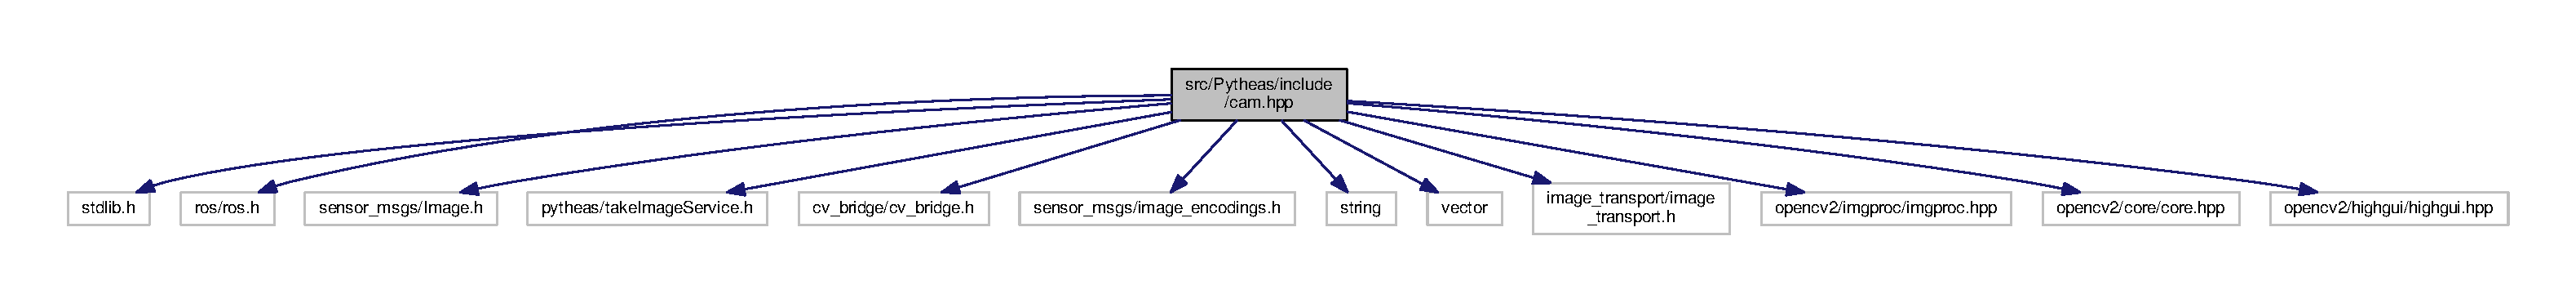
\includegraphics[width=350pt]{cam_8hpp__incl}
\end{center}
\end{figure}
This graph shows which files directly or indirectly include this file\+:
\nopagebreak
\begin{figure}[H]
\begin{center}
\leavevmode
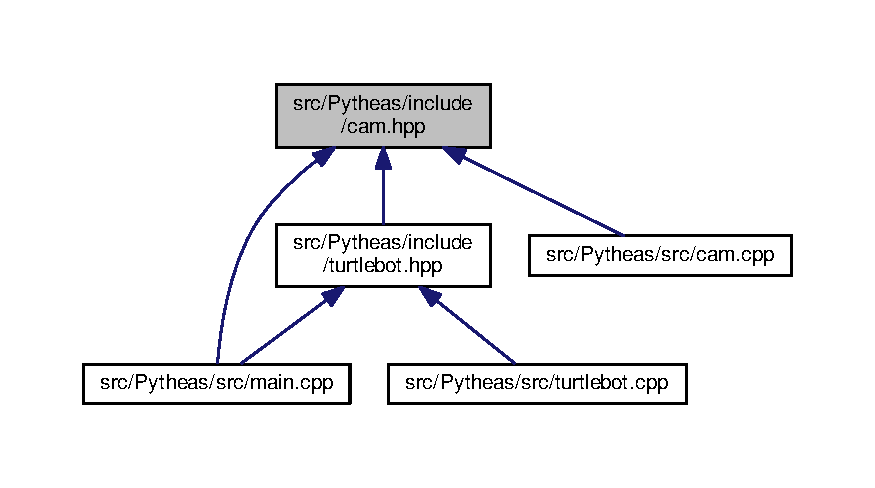
\includegraphics[width=350pt]{cam_8hpp__dep__incl}
\end{center}
\end{figure}
\subsection*{Classes}
\begin{DoxyCompactItemize}
\item 
class \hyperlink{class_cam}{Cam}
\begin{DoxyCompactList}\small\item\em \hyperlink{class_cam}{Cam} class handles viewing onboard imagery and taking images. \end{DoxyCompactList}\end{DoxyCompactItemize}


\subsection{Detailed Description}
Camera class definition. 

B\+SD 3-\/\+Clause License

Copyright (c) 2018, Yash Shah All rights reserved.

Redistribution and use in source and binary forms, with or without modification, are permitted provided that the following conditions are met\+:


\begin{DoxyItemize}
\item Redistributions of source code must retain the above copyright notice, this list of conditions and the following disclaimer.
\item Redistributions in binary form must reproduce the above copyright notice, this list of conditions and the following disclaimer in the documentation and/or other materials provided with the distribution.
\item Neither the name of the copyright holder nor the names of its contributors may be used to endorse or promote products derived from this software without specific prior written permission.
\end{DoxyItemize}

T\+H\+IS S\+O\+F\+T\+W\+A\+RE IS P\+R\+O\+V\+I\+D\+ED BY T\+HE C\+O\+P\+Y\+R\+I\+G\+HT H\+O\+L\+D\+E\+RS A\+ND C\+O\+N\+T\+R\+I\+B\+U\+T\+O\+RS \char`\"{}\+A\+S I\+S\char`\"{} A\+ND A\+NY E\+X\+P\+R\+E\+SS OR I\+M\+P\+L\+I\+ED W\+A\+R\+R\+A\+N\+T\+I\+ES, I\+N\+C\+L\+U\+D\+I\+NG, B\+UT N\+OT L\+I\+M\+I\+T\+ED TO, T\+HE I\+M\+P\+L\+I\+ED W\+A\+R\+R\+A\+N\+T\+I\+ES OF M\+E\+R\+C\+H\+A\+N\+T\+A\+B\+I\+L\+I\+TY A\+ND F\+I\+T\+N\+E\+SS F\+OR A P\+A\+R\+T\+I\+C\+U\+L\+AR P\+U\+R\+P\+O\+SE A\+RE D\+I\+S\+C\+L\+A\+I\+M\+ED. IN NO E\+V\+E\+NT S\+H\+A\+LL T\+HE C\+O\+P\+Y\+R\+I\+G\+HT H\+O\+L\+D\+ER OR C\+O\+N\+T\+R\+I\+B\+U\+T\+O\+RS BE L\+I\+A\+B\+LE F\+OR A\+NY D\+I\+R\+E\+CT, I\+N\+D\+I\+R\+E\+CT, I\+N\+C\+I\+D\+E\+N\+T\+AL, S\+P\+E\+C\+I\+AL, E\+X\+E\+M\+P\+L\+A\+RY, OR C\+O\+N\+S\+E\+Q\+U\+E\+N\+T\+I\+AL D\+A\+M\+A\+G\+ES (I\+N\+C\+L\+U\+D\+I\+NG, B\+UT N\+OT L\+I\+M\+I\+T\+ED TO, P\+R\+O\+C\+U\+R\+E\+M\+E\+NT OF S\+U\+B\+S\+T\+I\+T\+U\+TE G\+O\+O\+DS OR S\+E\+R\+V\+I\+C\+ES; L\+O\+SS OF U\+SE, D\+A\+TA, OR P\+R\+O\+F\+I\+TS; OR B\+U\+S\+I\+N\+E\+SS I\+N\+T\+E\+R\+R\+U\+P\+T\+I\+ON) H\+O\+W\+E\+V\+ER C\+A\+U\+S\+ED A\+ND ON A\+NY T\+H\+E\+O\+RY OF L\+I\+A\+B\+I\+L\+I\+TY, W\+H\+E\+T\+H\+ER IN C\+O\+N\+T\+R\+A\+CT, S\+T\+R\+I\+CT L\+I\+A\+B\+I\+L\+I\+TY, OR T\+O\+RT (I\+N\+C\+L\+U\+D\+I\+NG N\+E\+G\+L\+I\+G\+E\+N\+CE OR O\+T\+H\+E\+R\+W\+I\+SE) A\+R\+I\+S\+I\+NG IN A\+NY W\+AY O\+UT OF T\+HE U\+SE OF T\+H\+IS S\+O\+F\+T\+W\+A\+RE, E\+V\+EN IF A\+D\+V\+I\+S\+ED OF T\+HE P\+O\+S\+S\+I\+B\+I\+L\+I\+TY OF S\+U\+CH D\+A\+M\+A\+GE.

Yash Shah \begin{DoxyVersion}{Version}
1.\+0 Definition of the R\+OS Camera support methods.
\end{DoxyVersion}
\begin{DoxyCopyright}{Copyright}
B\+SD 3-\/\+Clause License 
\end{DoxyCopyright}

\hypertarget{control_motion_8hpp}{}\section{src/\+Pytheas/include/control\+Motion.hpp File Reference}
\label{control_motion_8hpp}\index{src/\+Pytheas/include/control\+Motion.\+hpp@{src/\+Pytheas/include/control\+Motion.\+hpp}}


\hyperlink{class_control_motion}{Control\+Motion} class definition.  


{\ttfamily \#include $<$stdlib.\+h$>$}\\*
{\ttfamily \#include $<$ros/ros.\+h$>$}\\*
{\ttfamily \#include $<$geometry\+\_\+msgs/\+Twist.\+h$>$}\\*
{\ttfamily \#include $<$sensor\+\_\+msgs/\+Laser\+Scan.\+h$>$}\\*
{\ttfamily \#include $<$pytheas/change\+Speed\+Service.\+h$>$}\\*
{\ttfamily \#include $<$pytheas/toggle\+Pause\+Motion.\+h$>$}\\*
{\ttfamily \#include $<$pytheas/change\+Threshold\+Service.\+h$>$}\\*
{\ttfamily \#include \char`\"{}detect\+Object.\+hpp\char`\"{}}\\*
{\ttfamily \#include \char`\"{}control\+Motion.\+hpp\char`\"{}}\\*
Include dependency graph for control\+Motion.\+hpp\+:
\nopagebreak
\begin{figure}[H]
\begin{center}
\leavevmode
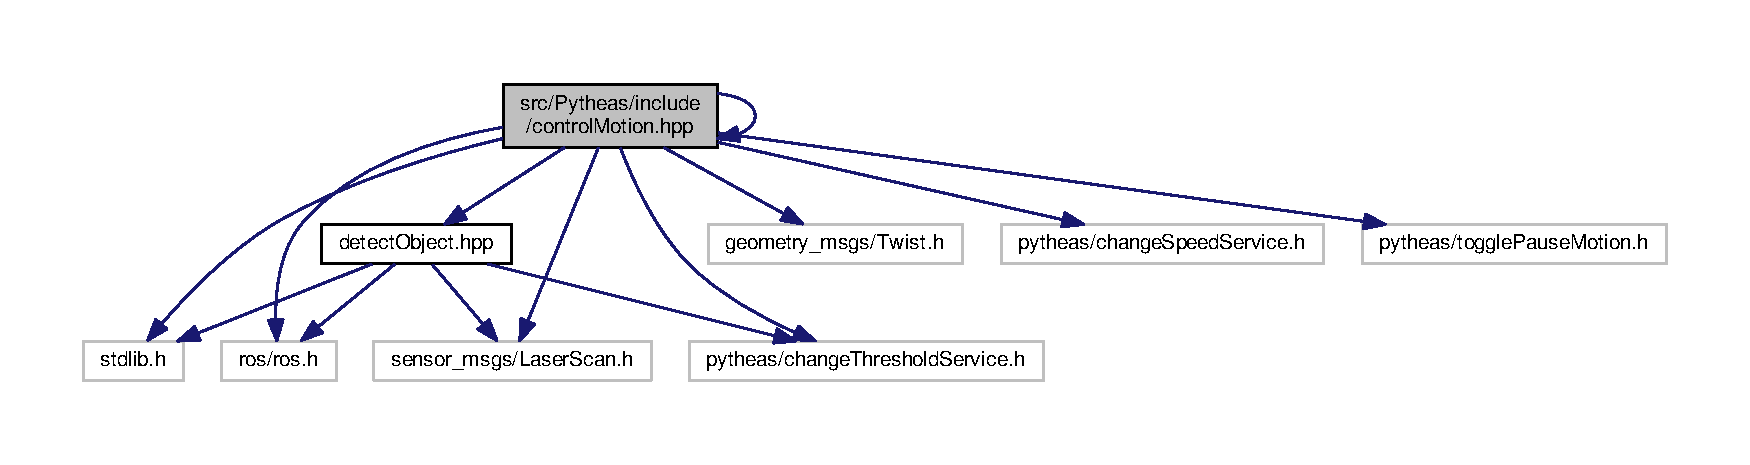
\includegraphics[width=350pt]{control_motion_8hpp__incl}
\end{center}
\end{figure}
This graph shows which files directly or indirectly include this file\+:
\nopagebreak
\begin{figure}[H]
\begin{center}
\leavevmode
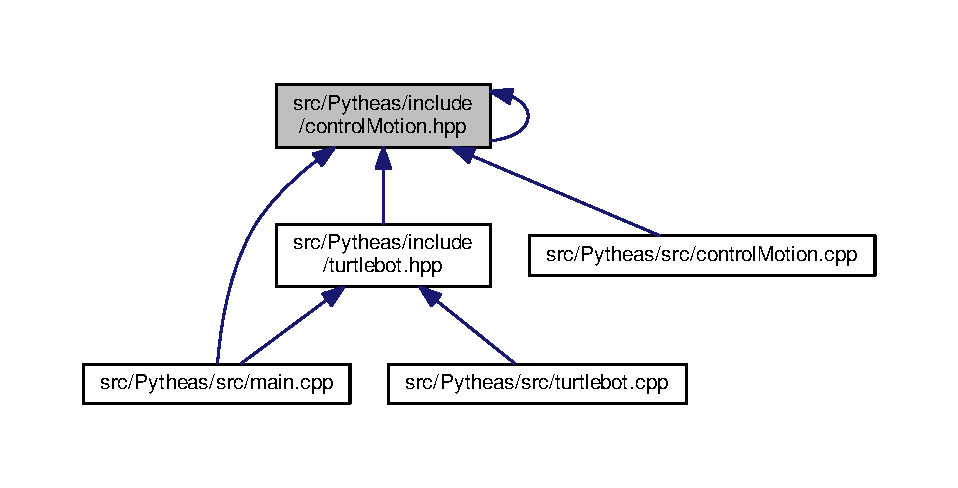
\includegraphics[width=350pt]{control_motion_8hpp__dep__incl}
\end{center}
\end{figure}
\subsection*{Classes}
\begin{DoxyCompactItemize}
\item 
class \hyperlink{class_control_motion}{Control\+Motion}
\begin{DoxyCompactList}\small\item\em control\+Motion class handles determining turtlebot control actions \end{DoxyCompactList}\end{DoxyCompactItemize}


\subsection{Detailed Description}
\hyperlink{class_control_motion}{Control\+Motion} class definition. 

B\+SD 3-\/\+Clause License

Copyright (c) 2018, Yash Shah All rights reserved.

Redistribution and use in source and binary forms, with or without modification, are permitted provided that the following conditions are met\+:


\begin{DoxyItemize}
\item Redistributions of source code must retain the above copyright notice, this list of conditions and the following disclaimer.
\item Redistributions in binary form must reproduce the above copyright notice, this list of conditions and the following disclaimer in the documentation and/or other materials provided with the distribution.
\item Neither the name of the copyright holder nor the names of its contributors may be used to endorse or promote products derived from this software without specific prior written permission.
\end{DoxyItemize}

T\+H\+IS S\+O\+F\+T\+W\+A\+RE IS P\+R\+O\+V\+I\+D\+ED BY T\+HE C\+O\+P\+Y\+R\+I\+G\+HT H\+O\+L\+D\+E\+RS A\+ND C\+O\+N\+T\+R\+I\+B\+U\+T\+O\+RS \char`\"{}\+A\+S I\+S\char`\"{} A\+ND A\+NY E\+X\+P\+R\+E\+SS OR I\+M\+P\+L\+I\+ED W\+A\+R\+R\+A\+N\+T\+I\+ES, I\+N\+C\+L\+U\+D\+I\+NG, B\+UT N\+OT L\+I\+M\+I\+T\+ED TO, T\+HE I\+M\+P\+L\+I\+ED W\+A\+R\+R\+A\+N\+T\+I\+ES OF M\+E\+R\+C\+H\+A\+N\+T\+A\+B\+I\+L\+I\+TY A\+ND F\+I\+T\+N\+E\+SS F\+OR A P\+A\+R\+T\+I\+C\+U\+L\+AR P\+U\+R\+P\+O\+SE A\+RE D\+I\+S\+C\+L\+A\+I\+M\+ED. IN NO E\+V\+E\+NT S\+H\+A\+LL T\+HE C\+O\+P\+Y\+R\+I\+G\+HT H\+O\+L\+D\+ER OR C\+O\+N\+T\+R\+I\+B\+U\+T\+O\+RS BE L\+I\+A\+B\+LE F\+OR A\+NY D\+I\+R\+E\+CT, I\+N\+D\+I\+R\+E\+CT, I\+N\+C\+I\+D\+E\+N\+T\+AL, S\+P\+E\+C\+I\+AL, E\+X\+E\+M\+P\+L\+A\+RY, OR C\+O\+N\+S\+E\+Q\+U\+E\+N\+T\+I\+AL D\+A\+M\+A\+G\+ES (I\+N\+C\+L\+U\+D\+I\+NG, B\+UT N\+OT L\+I\+M\+I\+T\+ED TO, P\+R\+O\+C\+U\+R\+E\+M\+E\+NT OF S\+U\+B\+S\+T\+I\+T\+U\+TE G\+O\+O\+DS OR S\+E\+R\+V\+I\+C\+ES; L\+O\+SS OF U\+SE, D\+A\+TA, OR P\+R\+O\+F\+I\+TS; OR B\+U\+S\+I\+N\+E\+SS I\+N\+T\+E\+R\+R\+U\+P\+T\+I\+ON) H\+O\+W\+E\+V\+ER C\+A\+U\+S\+ED A\+ND ON A\+NY T\+H\+E\+O\+RY OF L\+I\+A\+B\+I\+L\+I\+TY, W\+H\+E\+T\+H\+ER IN C\+O\+N\+T\+R\+A\+CT, S\+T\+R\+I\+CT L\+I\+A\+B\+I\+L\+I\+TY, OR T\+O\+RT (I\+N\+C\+L\+U\+D\+I\+NG N\+E\+G\+L\+I\+G\+E\+N\+CE OR O\+T\+H\+E\+R\+W\+I\+SE) A\+R\+I\+S\+I\+NG IN A\+NY W\+AY O\+UT OF T\+HE U\+SE OF T\+H\+IS S\+O\+F\+T\+W\+A\+RE, E\+V\+EN IF A\+D\+V\+I\+S\+ED OF T\+HE P\+O\+S\+S\+I\+B\+I\+L\+I\+TY OF S\+U\+CH D\+A\+M\+A\+GE.

Yash Shah \begin{DoxyVersion}{Version}
1.\+0 Definition of the R\+OS control\+Motion support methods.
\end{DoxyVersion}
\begin{DoxyCopyright}{Copyright}
B\+SD 3-\/\+Clause License 
\end{DoxyCopyright}

\hypertarget{detect_object_8hpp}{}\section{src/\+Pytheas/include/detect\+Object.hpp File Reference}
\label{detect_object_8hpp}\index{src/\+Pytheas/include/detect\+Object.\+hpp@{src/\+Pytheas/include/detect\+Object.\+hpp}}


\hyperlink{class_detect_object}{Detect\+Object} class definition.  


{\ttfamily \#include $<$stdlib.\+h$>$}\\*
{\ttfamily \#include $<$ros/ros.\+h$>$}\\*
{\ttfamily \#include $<$sensor\+\_\+msgs/\+Laser\+Scan.\+h$>$}\\*
{\ttfamily \#include $<$pytheas/change\+Threshold\+Service.\+h$>$}\\*
Include dependency graph for detect\+Object.\+hpp\+:
\nopagebreak
\begin{figure}[H]
\begin{center}
\leavevmode
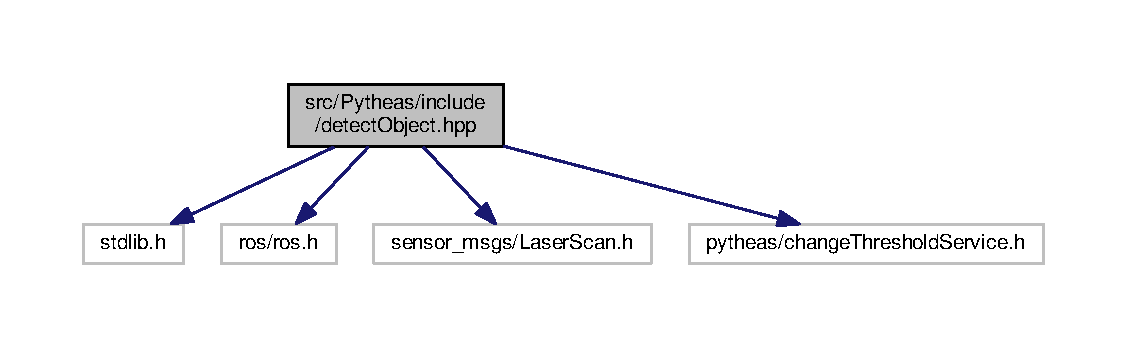
\includegraphics[width=350pt]{detect_object_8hpp__incl}
\end{center}
\end{figure}
This graph shows which files directly or indirectly include this file\+:
\nopagebreak
\begin{figure}[H]
\begin{center}
\leavevmode
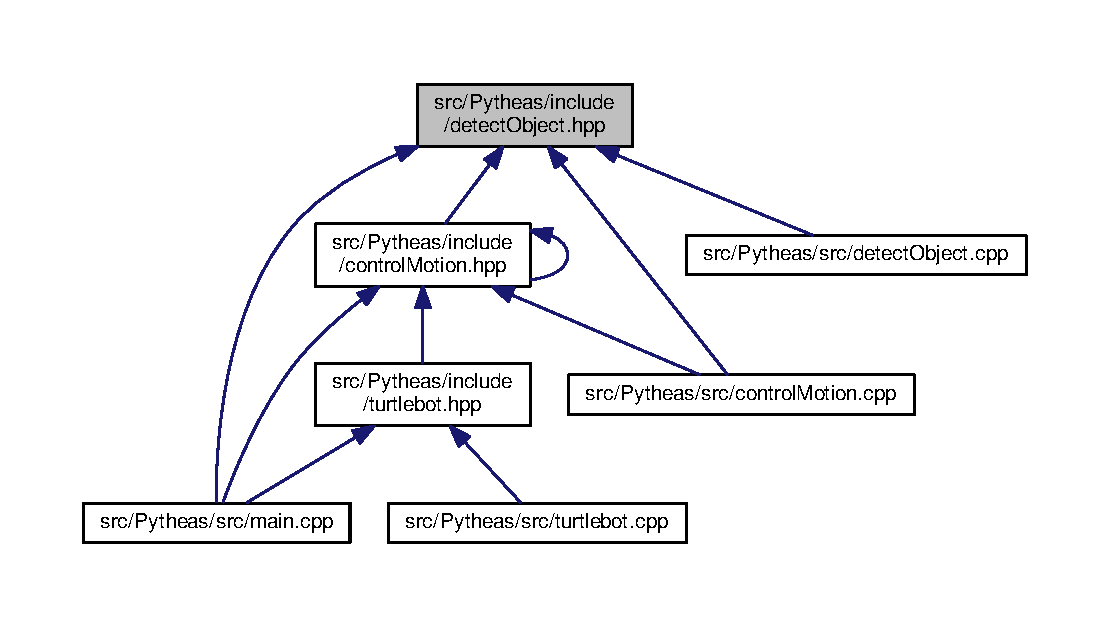
\includegraphics[width=350pt]{detect_object_8hpp__dep__incl}
\end{center}
\end{figure}
\subsection*{Classes}
\begin{DoxyCompactItemize}
\item 
class \hyperlink{class_detect_object}{Detect\+Object}
\begin{DoxyCompactList}\small\item\em detect\+Object class handles determining if the turtlebot is going to collide using laser scans \end{DoxyCompactList}\end{DoxyCompactItemize}


\subsection{Detailed Description}
\hyperlink{class_detect_object}{Detect\+Object} class definition. 

B\+SD 3-\/\+Clause License

Copyright (c) 2018, Yash Shah All rights reserved.

Redistribution and use in source and binary forms, with or without modification, are permitted provided that the following conditions are met\+:


\begin{DoxyItemize}
\item Redistributions of source code must retain the above copyright notice, this list of conditions and the following disclaimer.
\item Redistributions in binary form must reproduce the above copyright notice, this list of conditions and the following disclaimer in the documentation and/or other materials provided with the distribution.
\item Neither the name of the copyright holder nor the names of its contributors may be used to endorse or promote products derived from this software without specific prior written permission.
\end{DoxyItemize}

T\+H\+IS S\+O\+F\+T\+W\+A\+RE IS P\+R\+O\+V\+I\+D\+ED BY T\+HE C\+O\+P\+Y\+R\+I\+G\+HT H\+O\+L\+D\+E\+RS A\+ND C\+O\+N\+T\+R\+I\+B\+U\+T\+O\+RS \char`\"{}\+A\+S I\+S\char`\"{} A\+ND A\+NY E\+X\+P\+R\+E\+SS OR I\+M\+P\+L\+I\+ED W\+A\+R\+R\+A\+N\+T\+I\+ES, I\+N\+C\+L\+U\+D\+I\+NG, B\+UT N\+OT L\+I\+M\+I\+T\+ED TO, T\+HE I\+M\+P\+L\+I\+ED W\+A\+R\+R\+A\+N\+T\+I\+ES OF M\+E\+R\+C\+H\+A\+N\+T\+A\+B\+I\+L\+I\+TY A\+ND F\+I\+T\+N\+E\+SS F\+OR A P\+A\+R\+T\+I\+C\+U\+L\+AR P\+U\+R\+P\+O\+SE A\+RE D\+I\+S\+C\+L\+A\+I\+M\+ED. IN NO E\+V\+E\+NT S\+H\+A\+LL T\+HE C\+O\+P\+Y\+R\+I\+G\+HT H\+O\+L\+D\+ER OR C\+O\+N\+T\+R\+I\+B\+U\+T\+O\+RS BE L\+I\+A\+B\+LE F\+OR A\+NY D\+I\+R\+E\+CT, I\+N\+D\+I\+R\+E\+CT, I\+N\+C\+I\+D\+E\+N\+T\+AL, S\+P\+E\+C\+I\+AL, E\+X\+E\+M\+P\+L\+A\+RY, OR C\+O\+N\+S\+E\+Q\+U\+E\+N\+T\+I\+AL D\+A\+M\+A\+G\+ES (I\+N\+C\+L\+U\+D\+I\+NG, B\+UT N\+OT L\+I\+M\+I\+T\+ED TO, P\+R\+O\+C\+U\+R\+E\+M\+E\+NT OF S\+U\+B\+S\+T\+I\+T\+U\+TE G\+O\+O\+DS OR S\+E\+R\+V\+I\+C\+ES; L\+O\+SS OF U\+SE, D\+A\+TA, OR P\+R\+O\+F\+I\+TS; OR B\+U\+S\+I\+N\+E\+SS I\+N\+T\+E\+R\+R\+U\+P\+T\+I\+ON) H\+O\+W\+E\+V\+ER C\+A\+U\+S\+ED A\+ND ON A\+NY T\+H\+E\+O\+RY OF L\+I\+A\+B\+I\+L\+I\+TY, W\+H\+E\+T\+H\+ER IN C\+O\+N\+T\+R\+A\+CT, S\+T\+R\+I\+CT L\+I\+A\+B\+I\+L\+I\+TY, OR T\+O\+RT (I\+N\+C\+L\+U\+D\+I\+NG N\+E\+G\+L\+I\+G\+E\+N\+CE OR O\+T\+H\+E\+R\+W\+I\+SE) A\+R\+I\+S\+I\+NG IN A\+NY W\+AY O\+UT OF T\+HE U\+SE OF T\+H\+IS S\+O\+F\+T\+W\+A\+RE, E\+V\+EN IF A\+D\+V\+I\+S\+ED OF T\+HE P\+O\+S\+S\+I\+B\+I\+L\+I\+TY OF S\+U\+CH D\+A\+M\+A\+GE.

Yash Shah \begin{DoxyVersion}{Version}
1.\+0 Definition of the R\+OS detect\+Object support methods.
\end{DoxyVersion}
\begin{DoxyCopyright}{Copyright}
B\+SD 3-\/\+Clause License 
\end{DoxyCopyright}

\hypertarget{turtlebot_8hpp}{}\section{src/\+Pytheas/include/turtlebot.hpp File Reference}
\label{turtlebot_8hpp}\index{src/\+Pytheas/include/turtlebot.\+hpp@{src/\+Pytheas/include/turtlebot.\+hpp}}


\hyperlink{class_turtlebot}{Turtlebot} class definition.  


{\ttfamily \#include $<$stdlib.\+h$>$}\\*
{\ttfamily \#include $<$ros/ros.\+h$>$}\\*
{\ttfamily \#include $<$memory$>$}\\*
{\ttfamily \#include \char`\"{}control\+Motion.\+hpp\char`\"{}}\\*
{\ttfamily \#include \char`\"{}cam.\+hpp\char`\"{}}\\*
Include dependency graph for turtlebot.\+hpp\+:
\nopagebreak
\begin{figure}[H]
\begin{center}
\leavevmode
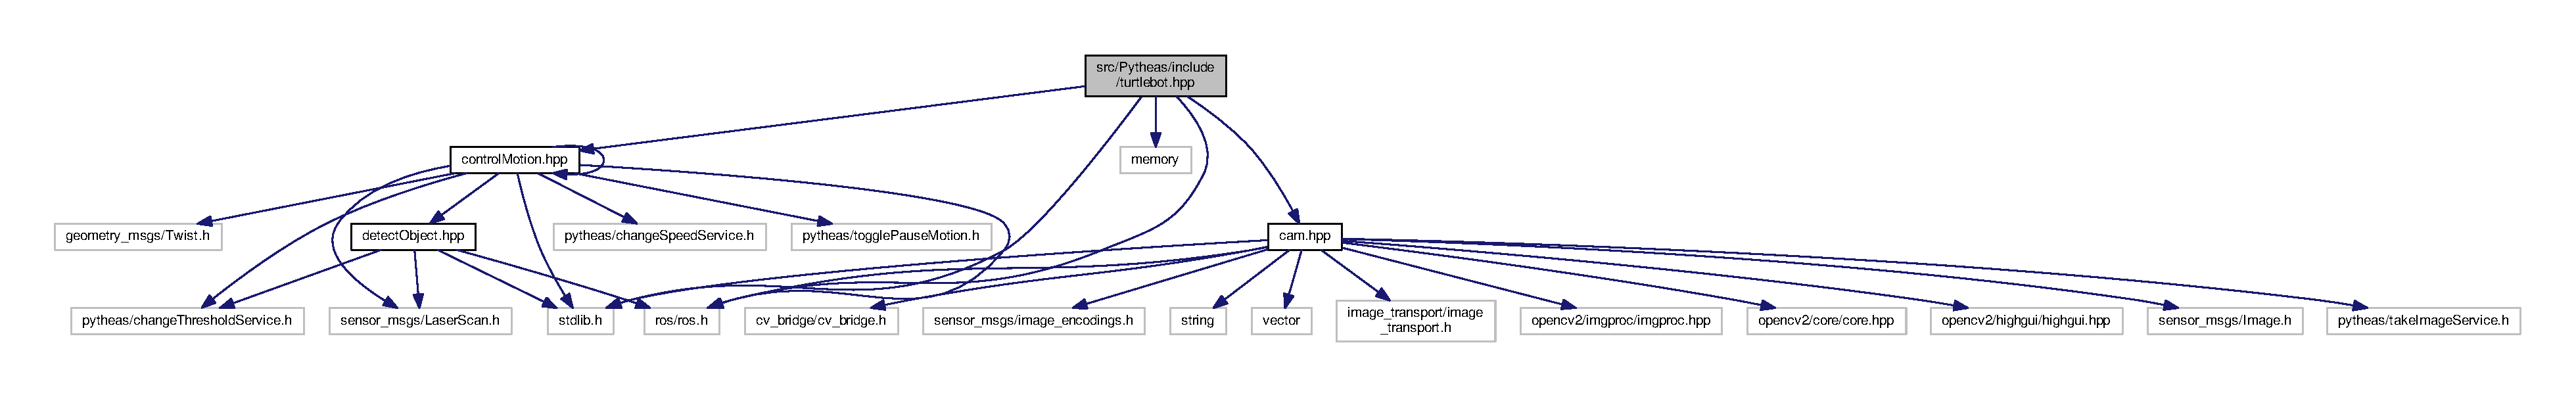
\includegraphics[width=350pt]{turtlebot_8hpp__incl}
\end{center}
\end{figure}
This graph shows which files directly or indirectly include this file\+:
\nopagebreak
\begin{figure}[H]
\begin{center}
\leavevmode
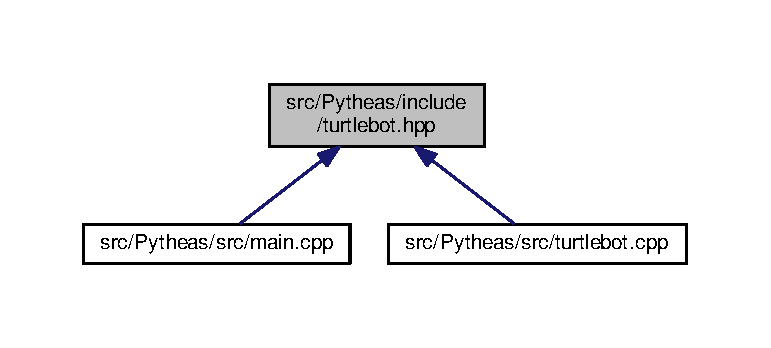
\includegraphics[width=350pt]{turtlebot_8hpp__dep__incl}
\end{center}
\end{figure}
\subsection*{Classes}
\begin{DoxyCompactItemize}
\item 
class \hyperlink{class_turtlebot}{Turtlebot}
\begin{DoxyCompactList}\small\item\em \hyperlink{class_turtlebot}{Turtlebot} class handles the camera and motion controller interactions for turtlebot. \end{DoxyCompactList}\end{DoxyCompactItemize}


\subsection{Detailed Description}
\hyperlink{class_turtlebot}{Turtlebot} class definition. 

B\+SD 3-\/\+Clause License

Copyright (c) 2018, Yash Shah All rights reserved.

Redistribution and use in source and binary forms, with or without modification, are permitted provided that the following conditions are met\+:


\begin{DoxyItemize}
\item Redistributions of source code must retain the above copyright notice, this list of conditions and the following disclaimer.
\item Redistributions in binary form must reproduce the above copyright notice, this list of conditions and the following disclaimer in the documentation and/or other materials provided with the distribution.
\item Neither the name of the copyright holder nor the names of its contributors may be used to endorse or promote products derived from this software without specific prior written permission.
\end{DoxyItemize}

T\+H\+IS S\+O\+F\+T\+W\+A\+RE IS P\+R\+O\+V\+I\+D\+ED BY T\+HE C\+O\+P\+Y\+R\+I\+G\+HT H\+O\+L\+D\+E\+RS A\+ND C\+O\+N\+T\+R\+I\+B\+U\+T\+O\+RS \char`\"{}\+A\+S I\+S\char`\"{} A\+ND A\+NY E\+X\+P\+R\+E\+SS OR I\+M\+P\+L\+I\+ED W\+A\+R\+R\+A\+N\+T\+I\+ES, I\+N\+C\+L\+U\+D\+I\+NG, B\+UT N\+OT L\+I\+M\+I\+T\+ED TO, T\+HE I\+M\+P\+L\+I\+ED W\+A\+R\+R\+A\+N\+T\+I\+ES OF M\+E\+R\+C\+H\+A\+N\+T\+A\+B\+I\+L\+I\+TY A\+ND F\+I\+T\+N\+E\+SS F\+OR A P\+A\+R\+T\+I\+C\+U\+L\+AR P\+U\+R\+P\+O\+SE A\+RE D\+I\+S\+C\+L\+A\+I\+M\+ED. IN NO E\+V\+E\+NT S\+H\+A\+LL T\+HE C\+O\+P\+Y\+R\+I\+G\+HT H\+O\+L\+D\+ER OR C\+O\+N\+T\+R\+I\+B\+U\+T\+O\+RS BE L\+I\+A\+B\+LE F\+OR A\+NY D\+I\+R\+E\+CT, I\+N\+D\+I\+R\+E\+CT, I\+N\+C\+I\+D\+E\+N\+T\+AL, S\+P\+E\+C\+I\+AL, E\+X\+E\+M\+P\+L\+A\+RY, OR C\+O\+N\+S\+E\+Q\+U\+E\+N\+T\+I\+AL D\+A\+M\+A\+G\+ES (I\+N\+C\+L\+U\+D\+I\+NG, B\+UT N\+OT L\+I\+M\+I\+T\+ED TO, P\+R\+O\+C\+U\+R\+E\+M\+E\+NT OF S\+U\+B\+S\+T\+I\+T\+U\+TE G\+O\+O\+DS OR S\+E\+R\+V\+I\+C\+ES; L\+O\+SS OF U\+SE, D\+A\+TA, OR P\+R\+O\+F\+I\+TS; OR B\+U\+S\+I\+N\+E\+SS I\+N\+T\+E\+R\+R\+U\+P\+T\+I\+ON) H\+O\+W\+E\+V\+ER C\+A\+U\+S\+ED A\+ND ON A\+NY T\+H\+E\+O\+RY OF L\+I\+A\+B\+I\+L\+I\+TY, W\+H\+E\+T\+H\+ER IN C\+O\+N\+T\+R\+A\+CT, S\+T\+R\+I\+CT L\+I\+A\+B\+I\+L\+I\+TY, OR T\+O\+RT (I\+N\+C\+L\+U\+D\+I\+NG N\+E\+G\+L\+I\+G\+E\+N\+CE OR O\+T\+H\+E\+R\+W\+I\+SE) A\+R\+I\+S\+I\+NG IN A\+NY W\+AY O\+UT OF T\+HE U\+SE OF T\+H\+IS S\+O\+F\+T\+W\+A\+RE, E\+V\+EN IF A\+D\+V\+I\+S\+ED OF T\+HE P\+O\+S\+S\+I\+B\+I\+L\+I\+TY OF S\+U\+CH D\+A\+M\+A\+GE.

Yash Shah \begin{DoxyVersion}{Version}
1.\+0 Definition of the R\+OS \hyperlink{class_turtlebot}{Turtlebot} support methods.
\end{DoxyVersion}
\begin{DoxyCopyright}{Copyright}
B\+SD 3-\/\+Clause License 
\end{DoxyCopyright}

\hypertarget{cam_8cpp}{}\section{src/\+Pytheas/src/cam.cpp File Reference}
\label{cam_8cpp}\index{src/\+Pytheas/src/cam.\+cpp@{src/\+Pytheas/src/cam.\+cpp}}


Camera class implementation.  


{\ttfamily \#include $<$stdlib.\+h$>$}\\*
{\ttfamily \#include $<$ros/ros.\+h$>$}\\*
{\ttfamily \#include $<$cv\+\_\+bridge/cv\+\_\+bridge.\+h$>$}\\*
{\ttfamily \#include $<$sensor\+\_\+msgs/image\+\_\+encodings.\+h$>$}\\*
{\ttfamily \#include $<$image\+\_\+transport/image\+\_\+transport.\+h$>$}\\*
{\ttfamily \#include $<$sstream$>$}\\*
{\ttfamily \#include $<$vector$>$}\\*
{\ttfamily \#include $<$string$>$}\\*
{\ttfamily \#include $<$opencv2/imgproc/imgproc.\+hpp$>$}\\*
{\ttfamily \#include $<$opencv2/core/core.\+hpp$>$}\\*
{\ttfamily \#include $<$opencv2/highgui/highgui.\+hpp$>$}\\*
{\ttfamily \#include \char`\"{}cam.\+hpp\char`\"{}}\\*
Include dependency graph for cam.\+cpp\+:
\nopagebreak
\begin{figure}[H]
\begin{center}
\leavevmode
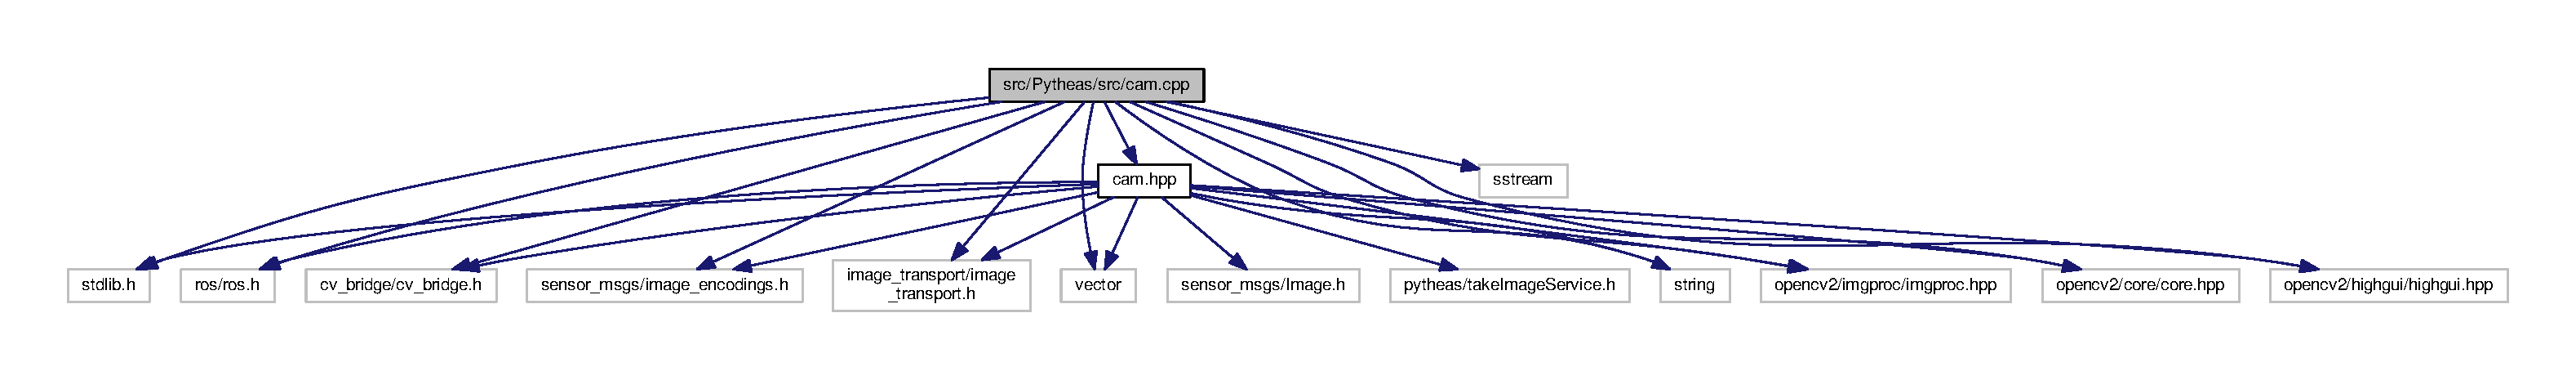
\includegraphics[width=350pt]{cam_8cpp__incl}
\end{center}
\end{figure}


\subsection{Detailed Description}
Camera class implementation. 

B\+SD 3-\/\+Clause License

Copyright (c) 2018, Yash Shah All rights reserved.

Redistribution and use in source and binary forms, with or without modification, are permitted provided that the following conditions are met\+:


\begin{DoxyItemize}
\item Redistributions of source code must retain the above copyright notice, this list of conditions and the following disclaimer.
\item Redistributions in binary form must reproduce the above copyright notice, this list of conditions and the following disclaimer in the documentation and/or other materials provided with the distribution.
\item Neither the name of the copyright holder nor the names of its contributors may be used to endorse or promote products derived from this software without specific prior written permission.
\end{DoxyItemize}

T\+H\+IS S\+O\+F\+T\+W\+A\+RE IS P\+R\+O\+V\+I\+D\+ED BY T\+HE C\+O\+P\+Y\+R\+I\+G\+HT H\+O\+L\+D\+E\+RS A\+ND C\+O\+N\+T\+R\+I\+B\+U\+T\+O\+RS \char`\"{}\+A\+S I\+S\char`\"{} A\+ND A\+NY E\+X\+P\+R\+E\+SS OR I\+M\+P\+L\+I\+ED W\+A\+R\+R\+A\+N\+T\+I\+ES, I\+N\+C\+L\+U\+D\+I\+NG, B\+UT N\+OT L\+I\+M\+I\+T\+ED TO, T\+HE I\+M\+P\+L\+I\+ED W\+A\+R\+R\+A\+N\+T\+I\+ES OF M\+E\+R\+C\+H\+A\+N\+T\+A\+B\+I\+L\+I\+TY A\+ND F\+I\+T\+N\+E\+SS F\+OR A P\+A\+R\+T\+I\+C\+U\+L\+AR P\+U\+R\+P\+O\+SE A\+RE D\+I\+S\+C\+L\+A\+I\+M\+ED. IN NO E\+V\+E\+NT S\+H\+A\+LL T\+HE C\+O\+P\+Y\+R\+I\+G\+HT H\+O\+L\+D\+ER OR C\+O\+N\+T\+R\+I\+B\+U\+T\+O\+RS BE L\+I\+A\+B\+LE F\+OR A\+NY D\+I\+R\+E\+CT, I\+N\+D\+I\+R\+E\+CT, I\+N\+C\+I\+D\+E\+N\+T\+AL, S\+P\+E\+C\+I\+AL, E\+X\+E\+M\+P\+L\+A\+RY, OR C\+O\+N\+S\+E\+Q\+U\+E\+N\+T\+I\+AL D\+A\+M\+A\+G\+ES (I\+N\+C\+L\+U\+D\+I\+NG, B\+UT N\+OT L\+I\+M\+I\+T\+ED TO, P\+R\+O\+C\+U\+R\+E\+M\+E\+NT OF S\+U\+B\+S\+T\+I\+T\+U\+TE G\+O\+O\+DS OR S\+E\+R\+V\+I\+C\+ES; L\+O\+SS OF U\+SE, D\+A\+TA, OR P\+R\+O\+F\+I\+TS; OR B\+U\+S\+I\+N\+E\+SS I\+N\+T\+E\+R\+R\+U\+P\+T\+I\+ON) H\+O\+W\+E\+V\+ER C\+A\+U\+S\+ED A\+ND ON A\+NY T\+H\+E\+O\+RY OF L\+I\+A\+B\+I\+L\+I\+TY, W\+H\+E\+T\+H\+ER IN C\+O\+N\+T\+R\+A\+CT, S\+T\+R\+I\+CT L\+I\+A\+B\+I\+L\+I\+TY, OR T\+O\+RT (I\+N\+C\+L\+U\+D\+I\+NG N\+E\+G\+L\+I\+G\+E\+N\+CE OR O\+T\+H\+E\+R\+W\+I\+SE) A\+R\+I\+S\+I\+NG IN A\+NY W\+AY O\+UT OF T\+HE U\+SE OF T\+H\+IS S\+O\+F\+T\+W\+A\+RE, E\+V\+EN IF A\+D\+V\+I\+S\+ED OF T\+HE P\+O\+S\+S\+I\+B\+I\+L\+I\+TY OF S\+U\+CH D\+A\+M\+A\+GE.

Yash Shah \begin{DoxyVersion}{Version}
1.\+0 Implementation of the R\+OS Camera support methods.
\end{DoxyVersion}
\begin{DoxyCopyright}{Copyright}
B\+SD 3-\/\+Clause License 
\end{DoxyCopyright}

\hypertarget{control_motion_8cpp}{}\section{src/\+Pytheas/src/control\+Motion.cpp File Reference}
\label{control_motion_8cpp}\index{src/\+Pytheas/src/control\+Motion.\+cpp@{src/\+Pytheas/src/control\+Motion.\+cpp}}


\hyperlink{class_control_motion}{Control\+Motion} class implementation.  


{\ttfamily \#include $<$stdlib.\+h$>$}\\*
{\ttfamily \#include $<$ros/ros.\+h$>$}\\*
{\ttfamily \#include $<$geometry\+\_\+msgs/\+Twist.\+h$>$}\\*
{\ttfamily \#include $<$sensor\+\_\+msgs/\+Laser\+Scan.\+h$>$}\\*
{\ttfamily \#include $<$pytheas/change\+Speed\+Service.\+h$>$}\\*
{\ttfamily \#include $<$pytheas/toggle\+Pause\+Motion.\+h$>$}\\*
{\ttfamily \#include $<$pytheas/change\+Threshold\+Service.\+h$>$}\\*
{\ttfamily \#include \char`\"{}detect\+Object.\+hpp\char`\"{}}\\*
{\ttfamily \#include \char`\"{}control\+Motion.\+hpp\char`\"{}}\\*
Include dependency graph for control\+Motion.\+cpp\+:
\nopagebreak
\begin{figure}[H]
\begin{center}
\leavevmode
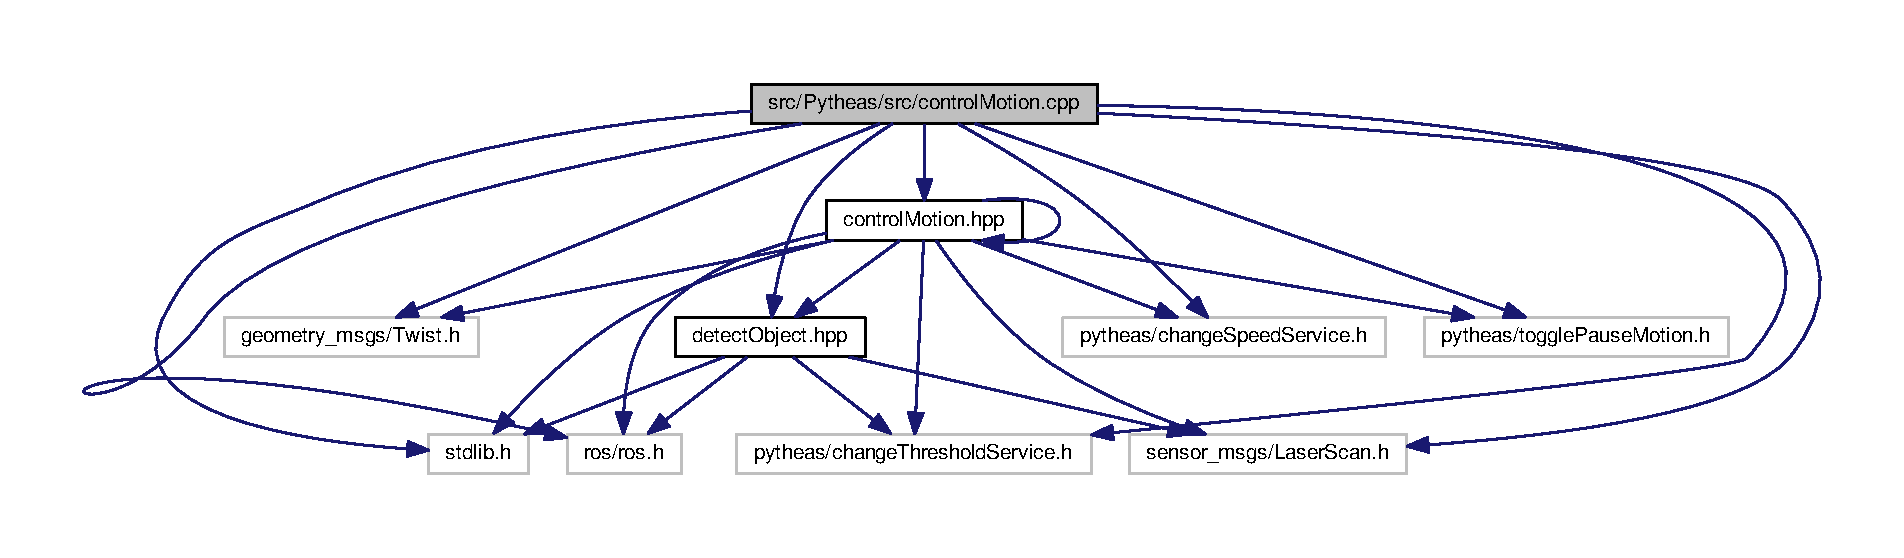
\includegraphics[width=350pt]{control_motion_8cpp__incl}
\end{center}
\end{figure}


\subsection{Detailed Description}
\hyperlink{class_control_motion}{Control\+Motion} class implementation. 

B\+SD 3-\/\+Clause License

Copyright (c) 2018, Yash Shah All rights reserved.

Redistribution and use in source and binary forms, with or without modification, are permitted provided that the following conditions are met\+:


\begin{DoxyItemize}
\item Redistributions of source code must retain the above copyright notice, this list of conditions and the following disclaimer.
\item Redistributions in binary form must reproduce the above copyright notice, this list of conditions and the following disclaimer in the documentation and/or other materials provided with the distribution.
\item Neither the name of the copyright holder nor the names of its contributors may be used to endorse or promote products derived from this software without specific prior written permission.
\end{DoxyItemize}

T\+H\+IS S\+O\+F\+T\+W\+A\+RE IS P\+R\+O\+V\+I\+D\+ED BY T\+HE C\+O\+P\+Y\+R\+I\+G\+HT H\+O\+L\+D\+E\+RS A\+ND C\+O\+N\+T\+R\+I\+B\+U\+T\+O\+RS \char`\"{}\+A\+S I\+S\char`\"{} A\+ND A\+NY E\+X\+P\+R\+E\+SS OR I\+M\+P\+L\+I\+ED W\+A\+R\+R\+A\+N\+T\+I\+ES, I\+N\+C\+L\+U\+D\+I\+NG, B\+UT N\+OT L\+I\+M\+I\+T\+ED TO, T\+HE I\+M\+P\+L\+I\+ED W\+A\+R\+R\+A\+N\+T\+I\+ES OF M\+E\+R\+C\+H\+A\+N\+T\+A\+B\+I\+L\+I\+TY A\+ND F\+I\+T\+N\+E\+SS F\+OR A P\+A\+R\+T\+I\+C\+U\+L\+AR P\+U\+R\+P\+O\+SE A\+RE D\+I\+S\+C\+L\+A\+I\+M\+ED. IN NO E\+V\+E\+NT S\+H\+A\+LL T\+HE C\+O\+P\+Y\+R\+I\+G\+HT H\+O\+L\+D\+ER OR C\+O\+N\+T\+R\+I\+B\+U\+T\+O\+RS BE L\+I\+A\+B\+LE F\+OR A\+NY D\+I\+R\+E\+CT, I\+N\+D\+I\+R\+E\+CT, I\+N\+C\+I\+D\+E\+N\+T\+AL, S\+P\+E\+C\+I\+AL, E\+X\+E\+M\+P\+L\+A\+RY, OR C\+O\+N\+S\+E\+Q\+U\+E\+N\+T\+I\+AL D\+A\+M\+A\+G\+ES (I\+N\+C\+L\+U\+D\+I\+NG, B\+UT N\+OT L\+I\+M\+I\+T\+ED TO, P\+R\+O\+C\+U\+R\+E\+M\+E\+NT OF S\+U\+B\+S\+T\+I\+T\+U\+TE G\+O\+O\+DS OR S\+E\+R\+V\+I\+C\+ES; L\+O\+SS OF U\+SE, D\+A\+TA, OR P\+R\+O\+F\+I\+TS; OR B\+U\+S\+I\+N\+E\+SS I\+N\+T\+E\+R\+R\+U\+P\+T\+I\+ON) H\+O\+W\+E\+V\+ER C\+A\+U\+S\+ED A\+ND ON A\+NY T\+H\+E\+O\+RY OF L\+I\+A\+B\+I\+L\+I\+TY, W\+H\+E\+T\+H\+ER IN C\+O\+N\+T\+R\+A\+CT, S\+T\+R\+I\+CT L\+I\+A\+B\+I\+L\+I\+TY, OR T\+O\+RT (I\+N\+C\+L\+U\+D\+I\+NG N\+E\+G\+L\+I\+G\+E\+N\+CE OR O\+T\+H\+E\+R\+W\+I\+SE) A\+R\+I\+S\+I\+NG IN A\+NY W\+AY O\+UT OF T\+HE U\+SE OF T\+H\+IS S\+O\+F\+T\+W\+A\+RE, E\+V\+EN IF A\+D\+V\+I\+S\+ED OF T\+HE P\+O\+S\+S\+I\+B\+I\+L\+I\+TY OF S\+U\+CH D\+A\+M\+A\+GE.

Yash Shah \begin{DoxyVersion}{Version}
1.\+0 Implementation of the R\+OS \hyperlink{class_control_motion}{Control\+Motion} support methods.
\end{DoxyVersion}
\begin{DoxyCopyright}{Copyright}
B\+SD 3-\/\+Clause License 
\end{DoxyCopyright}

\hypertarget{detect_object_8cpp}{}\section{src/\+Pytheas/src/detect\+Object.cpp File Reference}
\label{detect_object_8cpp}\index{src/\+Pytheas/src/detect\+Object.\+cpp@{src/\+Pytheas/src/detect\+Object.\+cpp}}


\hyperlink{class_detect_object}{Detect\+Object} class implementation.  


{\ttfamily \#include $<$stdlib.\+h$>$}\\*
{\ttfamily \#include $<$ros/ros.\+h$>$}\\*
{\ttfamily \#include $<$sensor\+\_\+msgs/\+Laser\+Scan.\+h$>$}\\*
{\ttfamily \#include $<$pytheas/change\+Threshold\+Service.\+h$>$}\\*
{\ttfamily \#include \char`\"{}detect\+Object.\+hpp\char`\"{}}\\*
Include dependency graph for detect\+Object.\+cpp\+:
\nopagebreak
\begin{figure}[H]
\begin{center}
\leavevmode
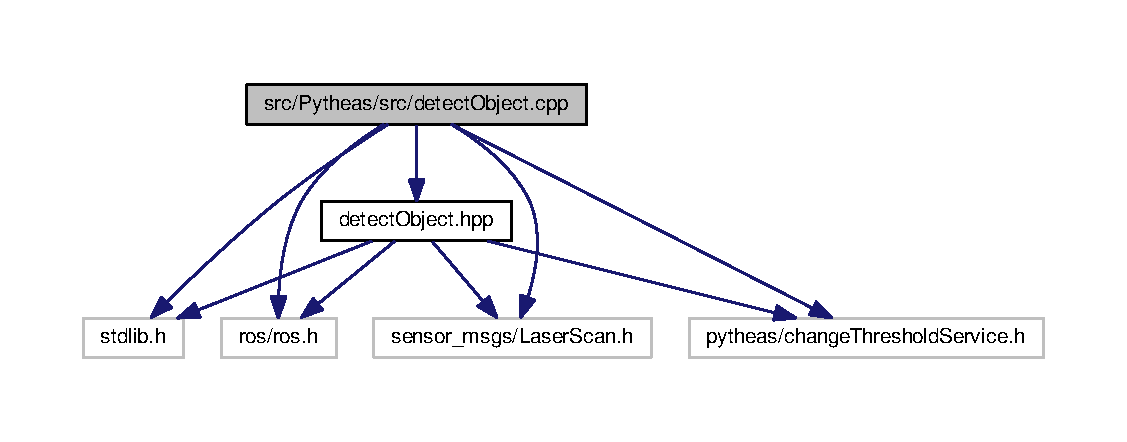
\includegraphics[width=350pt]{detect_object_8cpp__incl}
\end{center}
\end{figure}


\subsection{Detailed Description}
\hyperlink{class_detect_object}{Detect\+Object} class implementation. 

B\+SD 3-\/\+Clause License

Copyright (c) 2018, Yash Shah All rights reserved.

Redistribution and use in source and binary forms, with or without modification, are permitted provided that the following conditions are met\+:


\begin{DoxyItemize}
\item Redistributions of source code must retain the above copyright notice, this list of conditions and the following disclaimer.
\item Redistributions in binary form must reproduce the above copyright notice, this list of conditions and the following disclaimer in the documentation and/or other materials provided with the distribution.
\item Neither the name of the copyright holder nor the names of its contributors may be used to endorse or promote products derived from this software without specific prior written permission.
\end{DoxyItemize}

T\+H\+IS S\+O\+F\+T\+W\+A\+RE IS P\+R\+O\+V\+I\+D\+ED BY T\+HE C\+O\+P\+Y\+R\+I\+G\+HT H\+O\+L\+D\+E\+RS A\+ND C\+O\+N\+T\+R\+I\+B\+U\+T\+O\+RS \char`\"{}\+A\+S I\+S\char`\"{} A\+ND A\+NY E\+X\+P\+R\+E\+SS OR I\+M\+P\+L\+I\+ED W\+A\+R\+R\+A\+N\+T\+I\+ES, I\+N\+C\+L\+U\+D\+I\+NG, B\+UT N\+OT L\+I\+M\+I\+T\+ED TO, T\+HE I\+M\+P\+L\+I\+ED W\+A\+R\+R\+A\+N\+T\+I\+ES OF M\+E\+R\+C\+H\+A\+N\+T\+A\+B\+I\+L\+I\+TY A\+ND F\+I\+T\+N\+E\+SS F\+OR A P\+A\+R\+T\+I\+C\+U\+L\+AR P\+U\+R\+P\+O\+SE A\+RE D\+I\+S\+C\+L\+A\+I\+M\+ED. IN NO E\+V\+E\+NT S\+H\+A\+LL T\+HE C\+O\+P\+Y\+R\+I\+G\+HT H\+O\+L\+D\+ER OR C\+O\+N\+T\+R\+I\+B\+U\+T\+O\+RS BE L\+I\+A\+B\+LE F\+OR A\+NY D\+I\+R\+E\+CT, I\+N\+D\+I\+R\+E\+CT, I\+N\+C\+I\+D\+E\+N\+T\+AL, S\+P\+E\+C\+I\+AL, E\+X\+E\+M\+P\+L\+A\+RY, OR C\+O\+N\+S\+E\+Q\+U\+E\+N\+T\+I\+AL D\+A\+M\+A\+G\+ES (I\+N\+C\+L\+U\+D\+I\+NG, B\+UT N\+OT L\+I\+M\+I\+T\+ED TO, P\+R\+O\+C\+U\+R\+E\+M\+E\+NT OF S\+U\+B\+S\+T\+I\+T\+U\+TE G\+O\+O\+DS OR S\+E\+R\+V\+I\+C\+ES; L\+O\+SS OF U\+SE, D\+A\+TA, OR P\+R\+O\+F\+I\+TS; OR B\+U\+S\+I\+N\+E\+SS I\+N\+T\+E\+R\+R\+U\+P\+T\+I\+ON) H\+O\+W\+E\+V\+ER C\+A\+U\+S\+ED A\+ND ON A\+NY T\+H\+E\+O\+RY OF L\+I\+A\+B\+I\+L\+I\+TY, W\+H\+E\+T\+H\+ER IN C\+O\+N\+T\+R\+A\+CT, S\+T\+R\+I\+CT L\+I\+A\+B\+I\+L\+I\+TY, OR T\+O\+RT (I\+N\+C\+L\+U\+D\+I\+NG N\+E\+G\+L\+I\+G\+E\+N\+CE OR O\+T\+H\+E\+R\+W\+I\+SE) A\+R\+I\+S\+I\+NG IN A\+NY W\+AY O\+UT OF T\+HE U\+SE OF T\+H\+IS S\+O\+F\+T\+W\+A\+RE, E\+V\+EN IF A\+D\+V\+I\+S\+ED OF T\+HE P\+O\+S\+S\+I\+B\+I\+L\+I\+TY OF S\+U\+CH D\+A\+M\+A\+GE.

Yash Shah \begin{DoxyVersion}{Version}
1.\+0 Implementation of the R\+OS \hyperlink{class_detect_object}{Detect\+Object} support methods.
\end{DoxyVersion}
\begin{DoxyCopyright}{Copyright}
B\+SD 3-\/\+Clause License 
\end{DoxyCopyright}

\hypertarget{main_8cpp}{}\section{src/\+Pytheas/src/main.cpp File Reference}
\label{main_8cpp}\index{src/\+Pytheas/src/main.\+cpp@{src/\+Pytheas/src/main.\+cpp}}


main cpp file for the project repository  


{\ttfamily \#include $<$memory$>$}\\*
{\ttfamily \#include $<$stdlib.\+h$>$}\\*
{\ttfamily \#include $<$ros/ros.\+h$>$}\\*
{\ttfamily \#include \char`\"{}sensor\+\_\+msgs/\+Laser\+Scan.\+h\char`\"{}}\\*
{\ttfamily \#include \char`\"{}geometry\+\_\+msgs/\+Twist.\+h\char`\"{}}\\*
{\ttfamily \#include \char`\"{}sensor\+\_\+msgs/\+Image.\+h\char`\"{}}\\*
{\ttfamily \#include \char`\"{}turtlebot.\+hpp\char`\"{}}\\*
{\ttfamily \#include \char`\"{}cam.\+hpp\char`\"{}}\\*
{\ttfamily \#include \char`\"{}control\+Motion.\+hpp\char`\"{}}\\*
{\ttfamily \#include \char`\"{}detect\+Object.\+hpp\char`\"{}}\\*
Include dependency graph for main.\+cpp\+:
\nopagebreak
\begin{figure}[H]
\begin{center}
\leavevmode
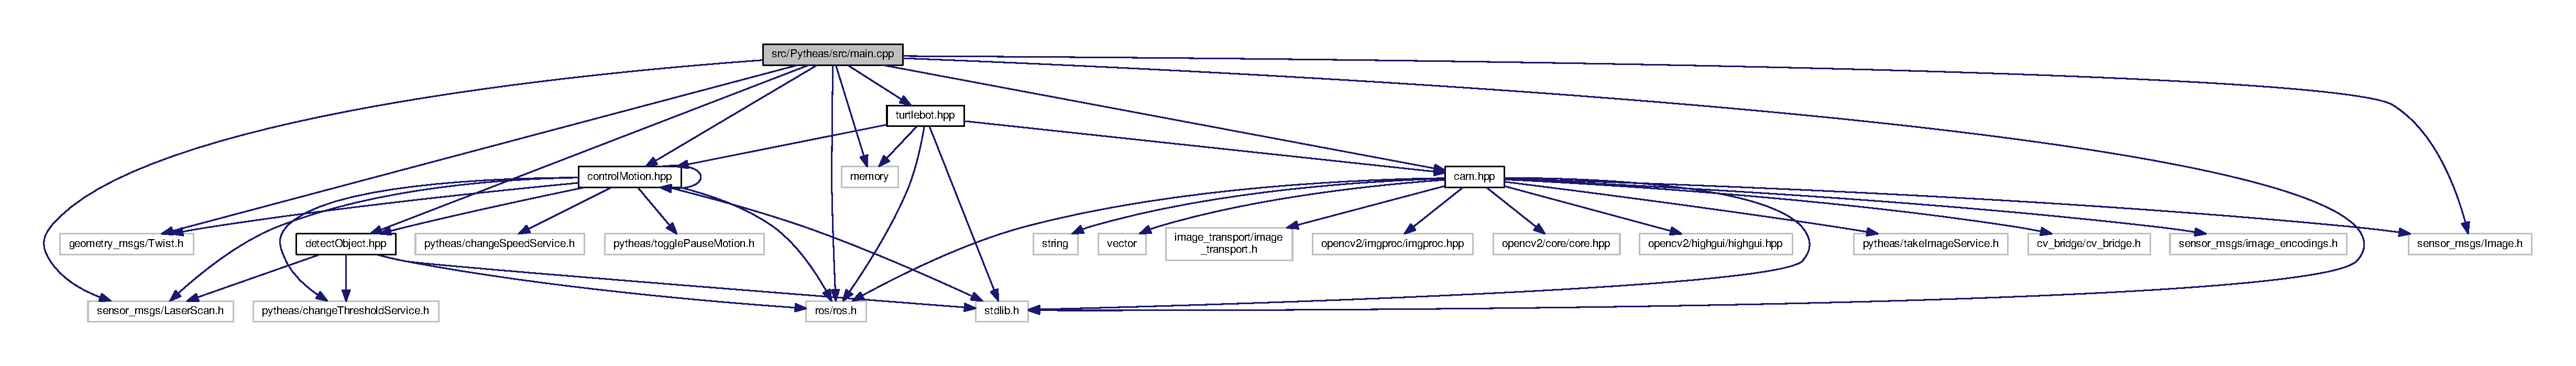
\includegraphics[width=350pt]{main_8cpp__incl}
\end{center}
\end{figure}
\subsection*{Functions}
\begin{DoxyCompactItemize}
\item 
int {\bfseries main} (int argc, char $\ast$$\ast$argv)\hypertarget{main_8cpp_a3c04138a5bfe5d72780bb7e82a18e627}{}\label{main_8cpp_a3c04138a5bfe5d72780bb7e82a18e627}

\end{DoxyCompactItemize}


\subsection{Detailed Description}
main cpp file for the project repository 

B\+SD 3-\/\+Clause License

Copyright (c) 2018, Yash Shah All rights reserved.

Redistribution and use in source and binary forms, with or without modification, are permitted provided that the following conditions are met\+:


\begin{DoxyItemize}
\item Redistributions of source code must retain the above copyright notice, this list of conditions and the following disclaimer.
\item Redistributions in binary form must reproduce the above copyright notice, this list of conditions and the following disclaimer in the documentation and/or other materials provided with the distribution.
\item Neither the name of the copyright holder nor the names of its contributors may be used to endorse or promote products derived from this software without specific prior written permission.
\end{DoxyItemize}

T\+H\+IS S\+O\+F\+T\+W\+A\+RE IS P\+R\+O\+V\+I\+D\+ED BY T\+HE C\+O\+P\+Y\+R\+I\+G\+HT H\+O\+L\+D\+E\+RS A\+ND C\+O\+N\+T\+R\+I\+B\+U\+T\+O\+RS \char`\"{}\+A\+S I\+S\char`\"{} A\+ND A\+NY E\+X\+P\+R\+E\+SS OR I\+M\+P\+L\+I\+ED W\+A\+R\+R\+A\+N\+T\+I\+ES, I\+N\+C\+L\+U\+D\+I\+NG, B\+UT N\+OT L\+I\+M\+I\+T\+ED TO, T\+HE I\+M\+P\+L\+I\+ED W\+A\+R\+R\+A\+N\+T\+I\+ES OF M\+E\+R\+C\+H\+A\+N\+T\+A\+B\+I\+L\+I\+TY A\+ND F\+I\+T\+N\+E\+SS F\+OR A P\+A\+R\+T\+I\+C\+U\+L\+AR P\+U\+R\+P\+O\+SE A\+RE D\+I\+S\+C\+L\+A\+I\+M\+ED. IN NO E\+V\+E\+NT S\+H\+A\+LL T\+HE C\+O\+P\+Y\+R\+I\+G\+HT H\+O\+L\+D\+ER OR C\+O\+N\+T\+R\+I\+B\+U\+T\+O\+RS BE L\+I\+A\+B\+LE F\+OR A\+NY D\+I\+R\+E\+CT, I\+N\+D\+I\+R\+E\+CT, I\+N\+C\+I\+D\+E\+N\+T\+AL, S\+P\+E\+C\+I\+AL, E\+X\+E\+M\+P\+L\+A\+RY, OR C\+O\+N\+S\+E\+Q\+U\+E\+N\+T\+I\+AL D\+A\+M\+A\+G\+ES (I\+N\+C\+L\+U\+D\+I\+NG, B\+UT N\+OT L\+I\+M\+I\+T\+ED TO, P\+R\+O\+C\+U\+R\+E\+M\+E\+NT OF S\+U\+B\+S\+T\+I\+T\+U\+TE G\+O\+O\+DS OR S\+E\+R\+V\+I\+C\+ES; L\+O\+SS OF U\+SE, D\+A\+TA, OR P\+R\+O\+F\+I\+TS; OR B\+U\+S\+I\+N\+E\+SS I\+N\+T\+E\+R\+R\+U\+P\+T\+I\+ON) H\+O\+W\+E\+V\+ER C\+A\+U\+S\+ED A\+ND ON A\+NY T\+H\+E\+O\+RY OF L\+I\+A\+B\+I\+L\+I\+TY, W\+H\+E\+T\+H\+ER IN C\+O\+N\+T\+R\+A\+CT, S\+T\+R\+I\+CT L\+I\+A\+B\+I\+L\+I\+TY, OR T\+O\+RT (I\+N\+C\+L\+U\+D\+I\+NG N\+E\+G\+L\+I\+G\+E\+N\+CE OR O\+T\+H\+E\+R\+W\+I\+SE) A\+R\+I\+S\+I\+NG IN A\+NY W\+AY O\+UT OF T\+HE U\+SE OF T\+H\+IS S\+O\+F\+T\+W\+A\+RE, E\+V\+EN IF A\+D\+V\+I\+S\+ED OF T\+HE P\+O\+S\+S\+I\+B\+I\+L\+I\+TY OF S\+U\+CH D\+A\+M\+A\+GE.

Yash Shah \begin{DoxyVersion}{Version}
1.\+0 This file is the main cpp file for the repository.
\end{DoxyVersion}
\begin{DoxyCopyright}{Copyright}
B\+SD 3-\/\+Clause License 
\end{DoxyCopyright}

\hypertarget{turtlebot_8cpp}{}\section{src/\+Pytheas/src/turtlebot.cpp File Reference}
\label{turtlebot_8cpp}\index{src/\+Pytheas/src/turtlebot.\+cpp@{src/\+Pytheas/src/turtlebot.\+cpp}}


\hyperlink{class_turtlebot}{Turtlebot} class implementation.  


{\ttfamily \#include $<$stdlib.\+h$>$}\\*
{\ttfamily \#include $<$ros/ros.\+h$>$}\\*
{\ttfamily \#include $<$geometry\+\_\+msgs/\+Twist.\+h$>$}\\*
{\ttfamily \#include $<$pytheas/take\+Image\+Service.\+h$>$}\\*
{\ttfamily \#include \char`\"{}turtlebot.\+hpp\char`\"{}}\\*
Include dependency graph for turtlebot.\+cpp\+:
\nopagebreak
\begin{figure}[H]
\begin{center}
\leavevmode
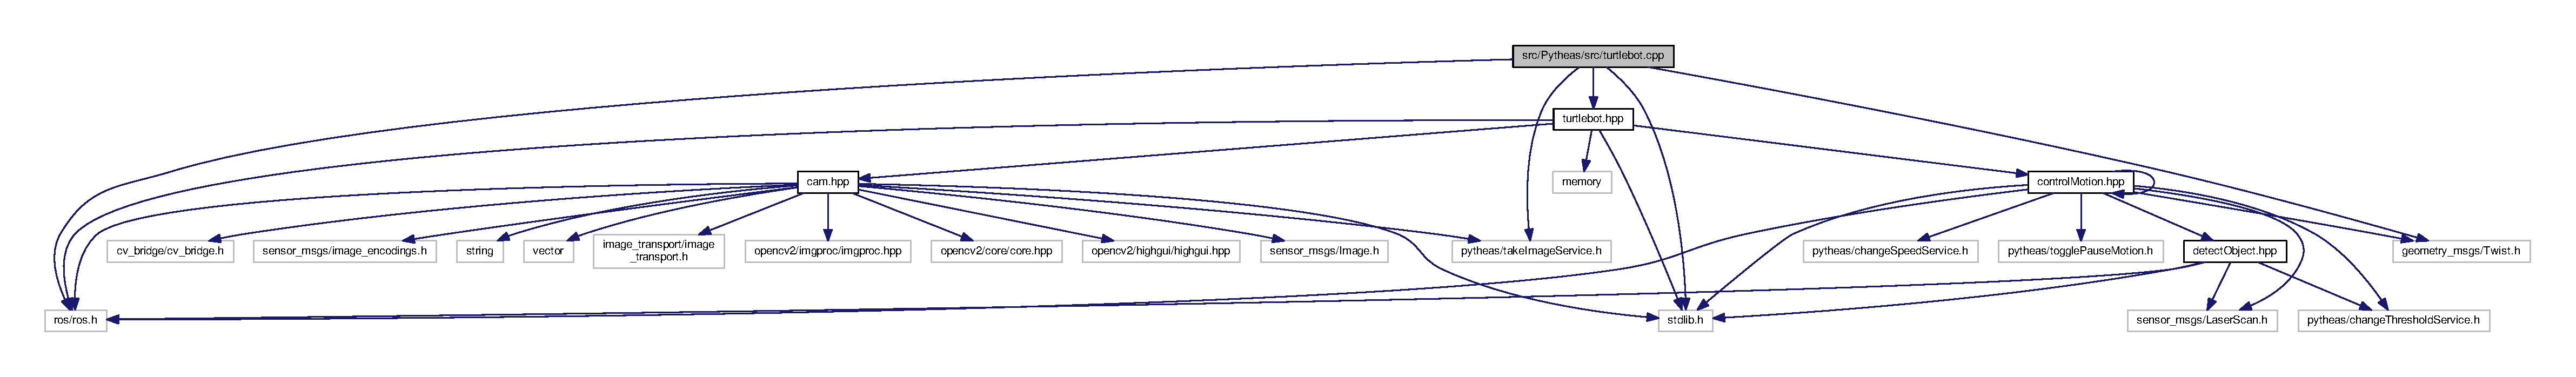
\includegraphics[width=350pt]{turtlebot_8cpp__incl}
\end{center}
\end{figure}


\subsection{Detailed Description}
\hyperlink{class_turtlebot}{Turtlebot} class implementation. 

B\+SD 3-\/\+Clause License

Copyright (c) 2018, Yash Shah All rights reserved.

Redistribution and use in source and binary forms, with or without modification, are permitted provided that the following conditions are met\+:


\begin{DoxyItemize}
\item Redistributions of source code must retain the above copyright notice, this list of conditions and the following disclaimer.
\item Redistributions in binary form must reproduce the above copyright notice, this list of conditions and the following disclaimer in the documentation and/or other materials provided with the distribution.
\item Neither the name of the copyright holder nor the names of its contributors may be used to endorse or promote products derived from this software without specific prior written permission.
\end{DoxyItemize}

T\+H\+IS S\+O\+F\+T\+W\+A\+RE IS P\+R\+O\+V\+I\+D\+ED BY T\+HE C\+O\+P\+Y\+R\+I\+G\+HT H\+O\+L\+D\+E\+RS A\+ND C\+O\+N\+T\+R\+I\+B\+U\+T\+O\+RS \char`\"{}\+A\+S I\+S\char`\"{} A\+ND A\+NY E\+X\+P\+R\+E\+SS OR I\+M\+P\+L\+I\+ED W\+A\+R\+R\+A\+N\+T\+I\+ES, I\+N\+C\+L\+U\+D\+I\+NG, B\+UT N\+OT L\+I\+M\+I\+T\+ED TO, T\+HE I\+M\+P\+L\+I\+ED W\+A\+R\+R\+A\+N\+T\+I\+ES OF M\+E\+R\+C\+H\+A\+N\+T\+A\+B\+I\+L\+I\+TY A\+ND F\+I\+T\+N\+E\+SS F\+OR A P\+A\+R\+T\+I\+C\+U\+L\+AR P\+U\+R\+P\+O\+SE A\+RE D\+I\+S\+C\+L\+A\+I\+M\+ED. IN NO E\+V\+E\+NT S\+H\+A\+LL T\+HE C\+O\+P\+Y\+R\+I\+G\+HT H\+O\+L\+D\+ER OR C\+O\+N\+T\+R\+I\+B\+U\+T\+O\+RS BE L\+I\+A\+B\+LE F\+OR A\+NY D\+I\+R\+E\+CT, I\+N\+D\+I\+R\+E\+CT, I\+N\+C\+I\+D\+E\+N\+T\+AL, S\+P\+E\+C\+I\+AL, E\+X\+E\+M\+P\+L\+A\+RY, OR C\+O\+N\+S\+E\+Q\+U\+E\+N\+T\+I\+AL D\+A\+M\+A\+G\+ES (I\+N\+C\+L\+U\+D\+I\+NG, B\+UT N\+OT L\+I\+M\+I\+T\+ED TO, P\+R\+O\+C\+U\+R\+E\+M\+E\+NT OF S\+U\+B\+S\+T\+I\+T\+U\+TE G\+O\+O\+DS OR S\+E\+R\+V\+I\+C\+ES; L\+O\+SS OF U\+SE, D\+A\+TA, OR P\+R\+O\+F\+I\+TS; OR B\+U\+S\+I\+N\+E\+SS I\+N\+T\+E\+R\+R\+U\+P\+T\+I\+ON) H\+O\+W\+E\+V\+ER C\+A\+U\+S\+ED A\+ND ON A\+NY T\+H\+E\+O\+RY OF L\+I\+A\+B\+I\+L\+I\+TY, W\+H\+E\+T\+H\+ER IN C\+O\+N\+T\+R\+A\+CT, S\+T\+R\+I\+CT L\+I\+A\+B\+I\+L\+I\+TY, OR T\+O\+RT (I\+N\+C\+L\+U\+D\+I\+NG N\+E\+G\+L\+I\+G\+E\+N\+CE OR O\+T\+H\+E\+R\+W\+I\+SE) A\+R\+I\+S\+I\+NG IN A\+NY W\+AY O\+UT OF T\+HE U\+SE OF T\+H\+IS S\+O\+F\+T\+W\+A\+RE, E\+V\+EN IF A\+D\+V\+I\+S\+ED OF T\+HE P\+O\+S\+S\+I\+B\+I\+L\+I\+TY OF S\+U\+CH D\+A\+M\+A\+GE.

Yash Shah \begin{DoxyVersion}{Version}
1.\+0 Implementation of the R\+OS \hyperlink{class_turtlebot}{Turtlebot} support methods.
\end{DoxyVersion}
\begin{DoxyCopyright}{Copyright}
B\+SD 3-\/\+Clause License 
\end{DoxyCopyright}

%--- End generated contents ---

% Index
\backmatter
\newpage
\phantomsection
\clearemptydoublepage
\addcontentsline{toc}{chapter}{Index}
\printindex

\end{document}
